\chapter{The effect of time costs on inquiry strategies}\label{ch:34}

\begin{mynote}
\subsubsection{Chapter outline}
%The previous chapter demonstrated that people adopt different strategies to address different inquiries. 
This chapter describes three controlled experiments that investigate the extent to which time costs of inquiries influence the number, duration and timing of inquiries for a data entry task. 

%Study 3 tests how IAC affects switching behaviour between one entry task and one information source. Study 4 tests switching behaviour between one entry task and multiple sources. Study 5 tests switching behaviour between multiple entry tasks and multiple sources.

Together these studies show that if the time cost of inquiries can be learnt in a controlled setting, participants adapt their behaviour to try and minimise time by reducing the number of inquiries with a high time cost, and postponing these to be addressed later, rather than addressing them immediately. 

\end{mynote}
 
 \section{Introduction}
The previous chapter revealed that office workers have different interruption strategies to address inquiries, and that there are different time costs associated with these inquiries. If information had to be retrieved from another physical location, participants postponed to access it later. However, digital interruptions were addressed immediately, as they were presumed to be quick. These interruptions could often take longer than intended, which suggests that people are not aware of time spent on digital interruptions. In the Discussion section of Study \hyperref[st:Study2]{2}, I considered whether making people more aware of time costs may help them in better managing their interruptions. However, it is not clear from the qualitative studies alone whether time costs actually influenced people's strategies, and what effect this has on task performance. This is important to understand, in order to know whether time information would be effective in managing inquiries and reducing their disruptiveness. Therefore, this chapter reports three lab experiments to study the effect of time costs on people's interruption behaviour in a controlled setting.

The aim of the studies reported in this chapter is to understand the effect of time costs on people's inquiry strategies for a data entry task. In particular, the first study of this chapter (Study \hyperref[st:Study3]{3}) aimed to investigate the effect of time costs on the \textit{number} and \textit{duration} of inquiries and task performance. The second study (Study \hyperref[st:Study4]{4}) aimed to investigate the effect of time costs on the \textit{timing} of inquiries. The aim of the third study (Study \hyperref[st:Study5]{5}) was to investigate the effect of time costs on timing of inquiries in a \textit{multi-task setup}.

To address the aims of this chapter, a controlled experimental study design was chosen as the study method, which is a useful method to measure the effect of changes of one variable on another variable \citep{Cairns2008}. To be able to study the effect of time costs on inquiry strategies, it was necessary to simplify the complexity of various time costs observed in Study \hyperref[st:Study2]{2} into a single independent variable that could easily be manipulated in a controlled environment. In this chapter, time costs are manipulated as the time effort to access task information: in each experiment, participants were given task information and had to copy this information into a data entry interface. Time costs were manipulated by including a time delay to reveal and perceive the information to-be-copied. This manipulation enabled people to learn the time costs associated with inquiries through interaction with the interface. Furthermore, it is a type of time cost which has been used in prior research \citep[e.g.][]{Gray2006, Morgan2009}, making it straightforward to compare the study findings with prior studies.

\newpage

\section{Study 3: Inquiries to a single source}\label{st:Study3}

\textit{A subset of the study sessions was run by Katherine Corneilson, an affiliate undergraduate student at UCL, as part of an undergraduate project. I designed the study, ran the majority of the sessions, and conducted the data analysis.}

\subsection{Introduction}
Participants in Study \hyperref[st:Study1]{1} and \hyperref[st:Study2]{2} had to retrieve and copy data from multiple sources with varying time costs for their work. Overall, participants were motivated to complete these tasks in an efficient manner: participants in Study  \hyperref[st:Study1]{1} said they held information in memory when between different computer windows, rather than writing it down. Furthermore, if participants in Study \hyperref[st:Study2]{2} knew they were going to need certain information, and knew there was a high time cost associated with getting this information, they prepared the information before starting a data entry task. 

The finding that participants tried to complete tasks efficiently is in line with the soft constraints hypothesis, a cognitive theory which states that people adapt their cognitive strategies to the constraints of a task environment with the aim to optimise task completion time \citep{Gray2006}. This theory has been tested through a series of lab experiments that manipulated the cost to access task information. These studies have consistently shown that as the cost to access task information increases, people try to minimise interruptions to access task information, and instead rely on information they have memorised. Relying on memory may be a good strategy: making fewer interruptions is less disruptive, and people are quicker to resume the task after being away, because task information is still in memory \citep{Morgan2009}. However, the effect of this strategy on task performance differed across studies: while in some studies it made people more efficient and accurate, in others it slowed people down and increased errors. 

For example, \citet{Waldron2007} used a flight simulation task in their study, in which participants had to use flight information to navigate aircraft to sites of interest. If there was a high time cost associated with accessing task information, participants increasingly relied on information in memory, and were more efficient to complete the task, as they did not have to interrupt their task as often to look back at the information. 

\newpage

\citet{Gray2004} conducted an experiment where people had to copy over VCR programming information. Participants either had permanent access to the information, or they were explicitly instructed and trained before the trial to memorise the information. In the latter condition, the information during the trial was covered by a grey box which could be uncovered by hovering over it with the cursor. The people in the latter condition were more accurate than the other condition in entering the information. These studies showed that a memory-intensive strategy to save time can improve task performance, if the information is well-encoded in memory.

However, other studies instead found a decrease of task performance when the cost to access task information was increased \citep{Gray2006, Morgan2009}. In these studies, the Blocks World Task (BWT) was used as a task paradigm, which requires people to copy a 3x3 pattern of coloured blocks, by dragging blocks from a resource window to a target window and putting them in the correct order. The cost to access task information was manipulated across three conditions. In the Low Cost condition, the pattern was permanently visible on the screen. In the Medium Cost condition, the pattern was covered by a grey mask and participants had to hover over the mask with their mouse to reveal the pattern. In the High Cost condition, there was a 2.5 second delay before the pattern was revealed. As in prior studies, participants made fewer interruptions to access information if there was a time cost associated, and instead relied on information in memory. Looking at overall task performance however, they made more errors and took considerably longer to complete the task. In a later paper, the researchers reflected that the coloured blocks participants had to copy may have been too demanding to memorise \citep{Waldron2011}. This abstract visuo-spatial information did not bear any meaning to the participant, in contrast with the VCR programming information used in \citet{Gray2004} and the flight information used in \citet{Waldron2007} which resembles more familiar information used in a real-world task, and is easier to memorise.

The different effect of a memory-intensive strategy on task performance across studies suggests that the type of task information matters: if information is easy to remember, a memory-based strategy makes it better encoded in memory, with improved task performance as a result. However the studies discussed above not only differed in type of task information they used, but also in task paradigm, which makes it hard to compare their findings and say for certain the difference in results is due to the information: for instance, in \citet{Gray2004} people were explicitly instructed to memorise the information and completed a test prior to a trial during which they had to fill in the information, and could not continue until they had stated everything correctly. This instruction ensured that people had the information well-memorised before they started the experimental trial. In the Blocks World Task studies, participants were not trained or instructed to memorise information well.

It is important to not only understand to what extent people avoid time costs during a task, but also what effect this has on their task performance. Therefore Study \hyperref[st:Study3]{3} first replicates the BWT and only changes type of information, with the aim to see whether the effect of time costs on task performance depends on the type of task information. Study \hyperref[st:Study3]{3} is the only study in the thesis that uses this task paradigm, which was necessary to make a comparison with findings from previous work. The remainder of the thesis uses an expenses task which is based on the type of expenses work observed in Study \hyperref[st:Study1]{1} and \hyperref[st:Study2]{2}. 

The aim of this study is to test the following hypotheses:

\begin{itemize}
\item [H1.]
As IAC increases, people will make fewer visits to the target window. 
\item [H2.]
As IAC increases, people will make longer visits to the target window.
\item [H3.]
As IAC increases, people in the Numbers condition will adapt their strategies and be faster to complete the task.
\item [H4.]
As IAC increases, people in the Numbers condition will make fewer errors.
\end{itemize}

\subsection{Method}
\subsubsection{Participants}
Fourty-two participants (34 female, eight male) were recruited from the UCL Psychology Subject Pool. Ages ranged from 18 to 52 (M = 22.38, SD = 7.45). Participants received course credit or \pounds3.75 as compensation for taking part in the study. 

\subsubsection{Materials}
Figure \ref{fig:ch4_taskparadigm} shows the task paradigm that was used. Each colour or number was only used once. The colours used were similar to the colours used in previous BWT studies \citep[e.g.][]{Gray2006, Morgan2009}, and were red, dark blue, green, yellow, black, pink, grey, light blue, orange, and purple.
Participants had to copy and complete fifteen patterns of each block type, and each participant had to copy over the same patterns. The target window showed a 3x3 grid with either coloured or numbered blocks. The output window showed an empty 3x3 grid, and was the same size as the target window. Participants had to copy the pattern shown in the target window by dragging blocks from the resource window and moving them into the output window. 

\begin{figure}[]
\begin{center}

\begin{subfigure}[b]{\textwidth}
\centerline{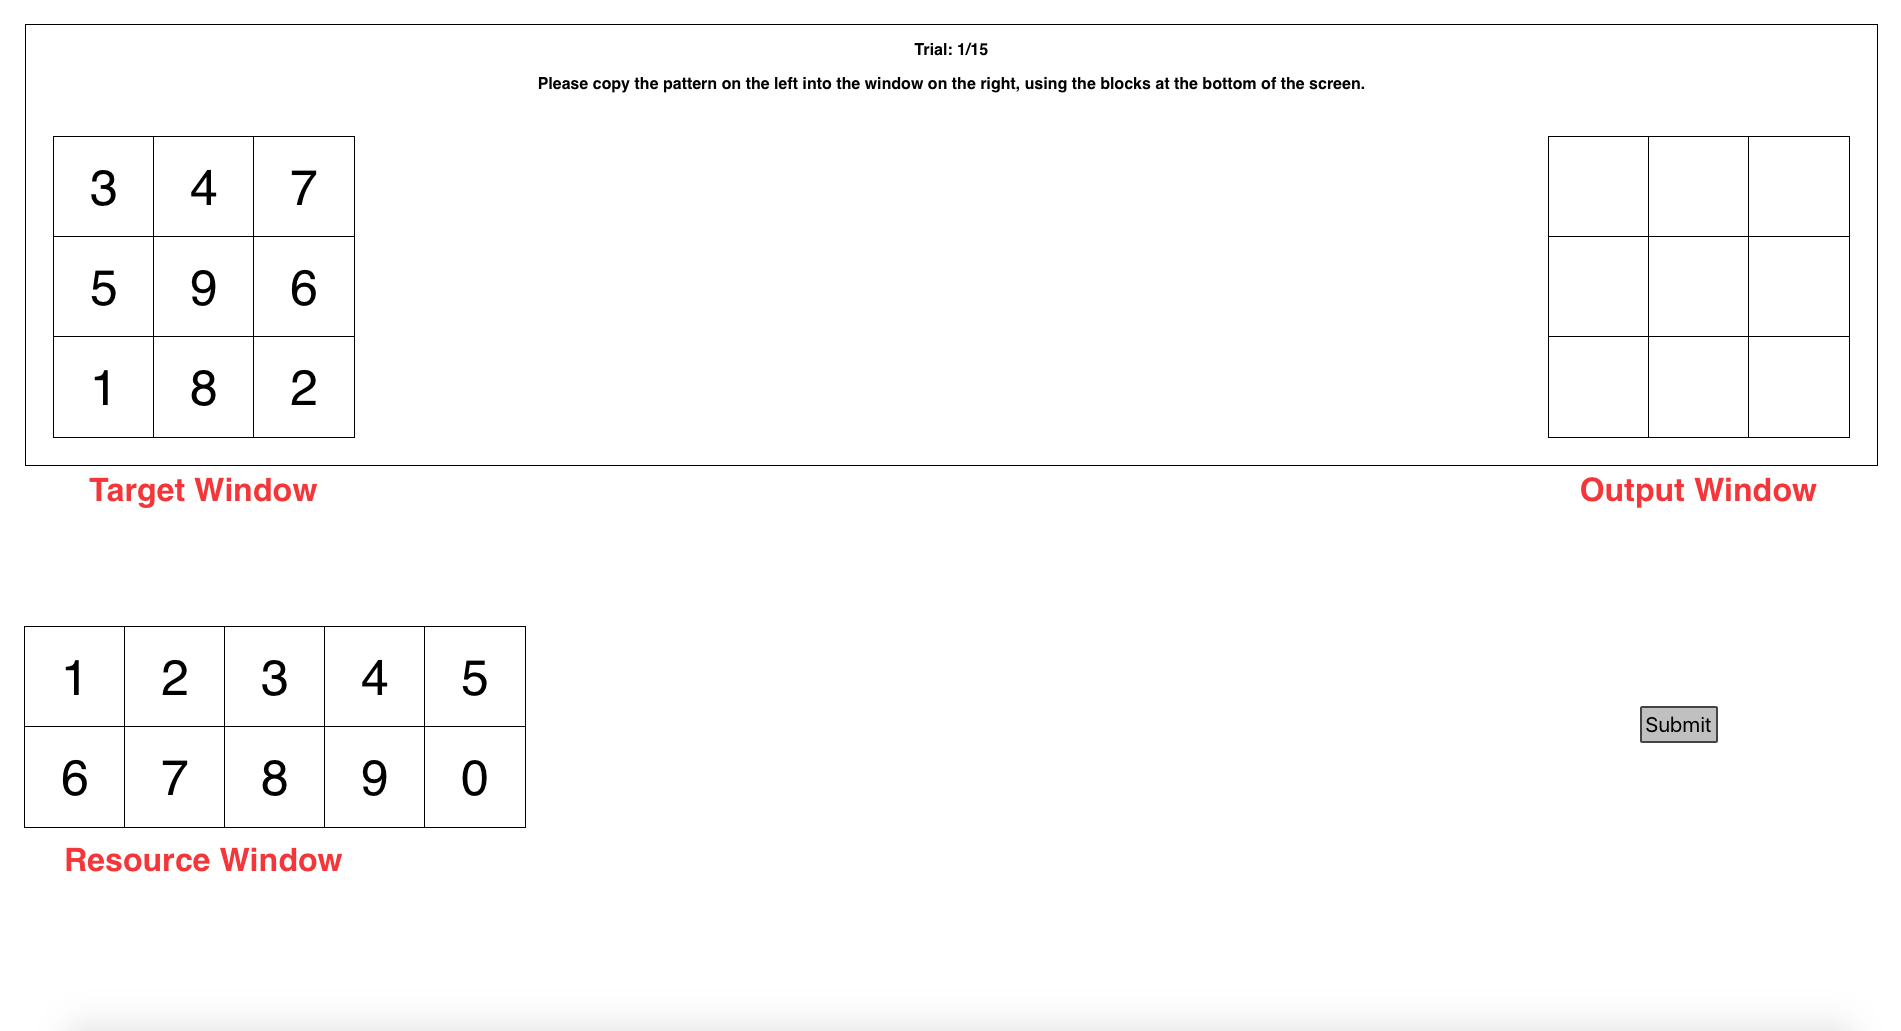
\includegraphics[scale=0.23]{images/ch34/ch4_numbers.png}}
\caption{The number condition.}
\label{fig:ch4_BWT}
\end{subfigure}
%\hfill%
\begin{subfigure}[b]{0.5\textwidth}
\centerline{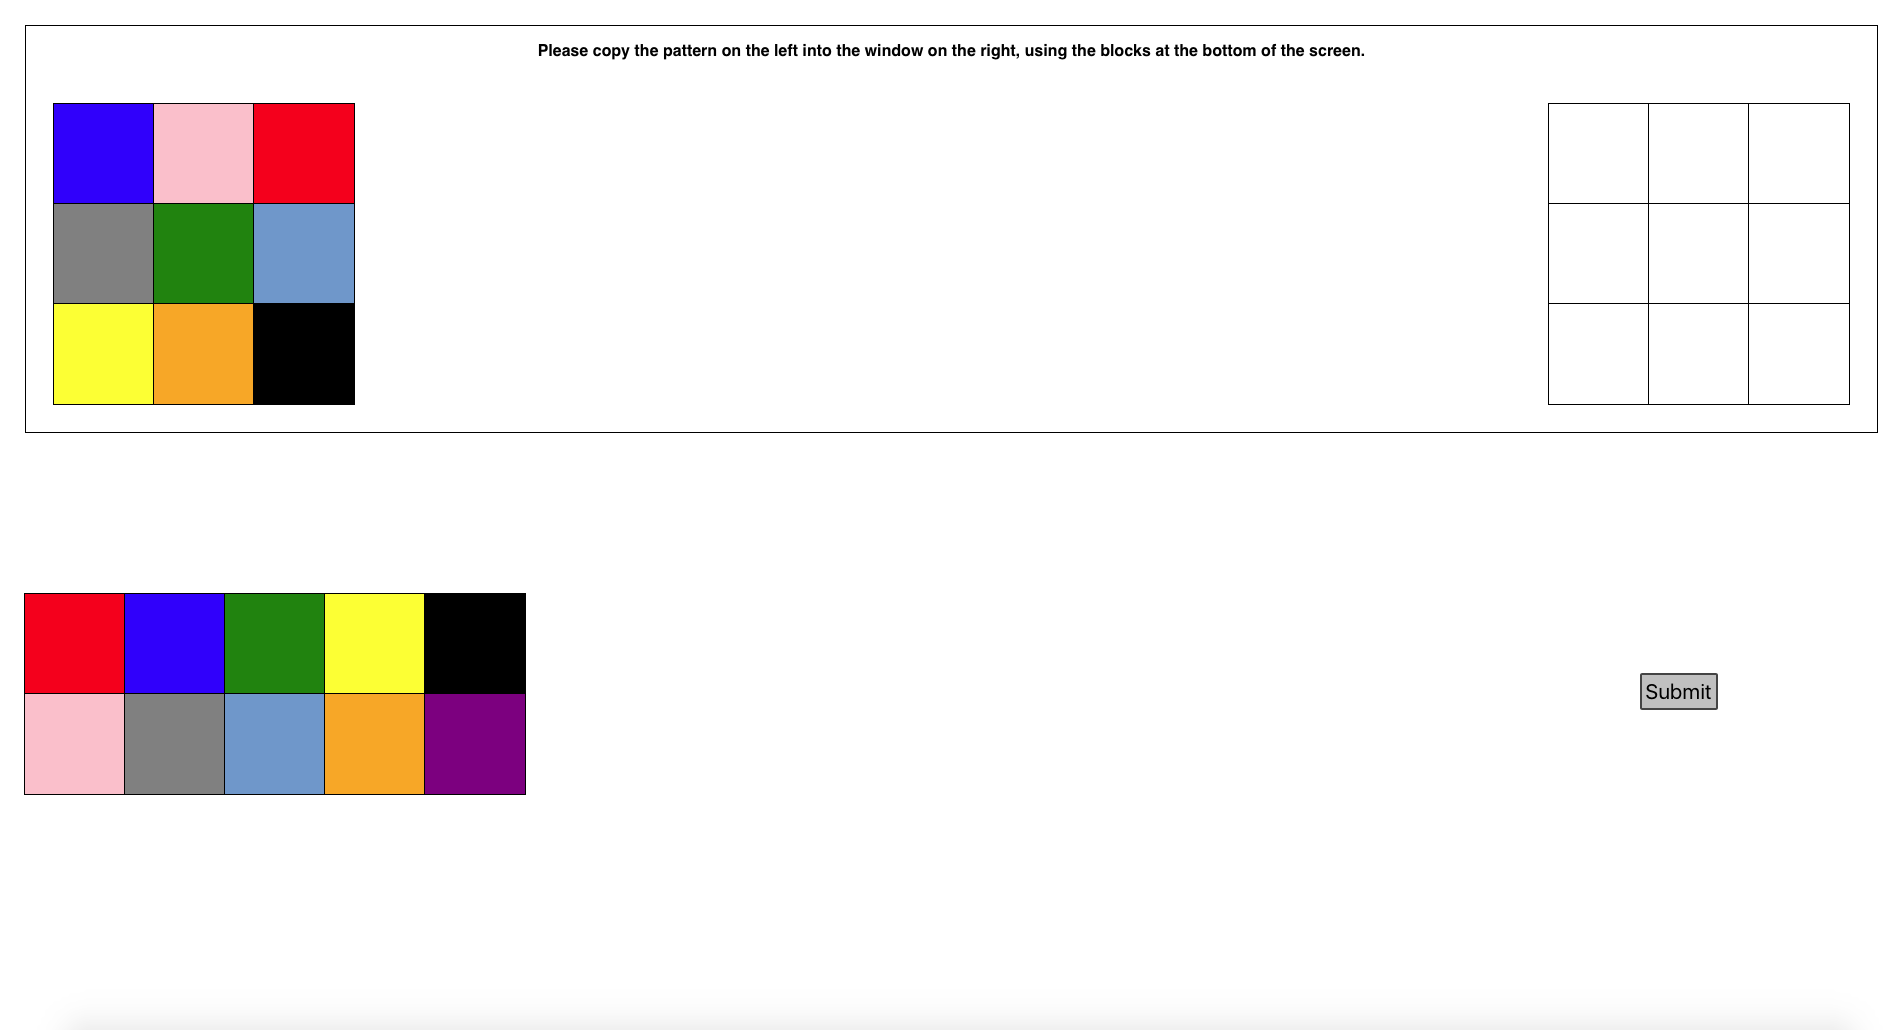
\includegraphics[scale=0.23]{images/ch34/ch4_colours.png}}
\caption{The colour condition.}
\label{fig:ch4_NWT}
\end{subfigure}
\caption[Study 3 task lay-out]{The task lay-out with the three different components. In the Medium and High IAC conditions, the Target Window was covered with a grey mask.}
\label{fig:ch4_taskparadigm}
\end{center}
\end{figure}

The study was conducted on a desktop computer, using a 24-inch monitor with a resolution of 2048 x 1152 pixels. Participants used a computer mouse to drag and drop blocks. The experimental task was implemented using HTML, JavaScript and PHP and run in a browser.  All relevant browser events, such as mouse movements to (un)cover the grey mask, dragging and dropping the blocks and mouse clicks, were recorded and saved in a mySQL database. The browser window covered the whole screen to minimise distractions.

A Tobii T60 eye tracker was used for recording people's eye fixations. Eye movements were recorded at a rate of 60 gaze data points per second for each eye, with an accuracy of 0.5 degrees and timestamp accuracy of 4 ms. For the analysis, all consecutive eye fixations with no drag or drop actions in-between were added together and counted as one fixation.

\subsubsection{Design}
A mixed design was used with two independent variables: time cost and block type. The between-participants variable was the level of time cost which had three levels. If the Cost was Low, the target pattern was permanently visible. In the Medium and High Cost conditions, the target pattern was covered with a grey mask, and could only be uncovered by moving the mouse cursor over the window. The mask reappeared as soon as the cursor left the window. In the High Cost condition, there was an additional 1-second delay to uncover the mask. This delay time was used in previous BWT studies where it showed to have a significant effect on task strategies and performance \citep{Gray2006, Morgan2009, Waldron2007}. The within-participants variable was the block type to be copied, which was either coloured or numbered blocks. The order was counter-balanced across participants.

The dependent variables are listed in Table \ref{table:ch4_dvs}. For the Low Cost condition, the number and duration of visits to the target window were measured using eye fixations; consecutive eye movements within the target area were counted as one visit. Eye-tracking data was also obtained for the Medium and High Cost conditions. However, this eye-tracking data was not used for these conditions, as people were able to look at the target window area without uncovering and perceiving the target pattern. Therefore, in accordance with previous studies \citep{Morgan2009, Patrick2014, Waldron2007, Waldron2011}, for the Medium and High Cost conditions the frequency with which the target pattern was uncovered was used as a measurement for visits to the target window. These uncoverings were measured using JavaScript. Both the usefulness and limitations of using these measures are discussed in the Discussion.
 
 \begin{table}[htp]
\centering
 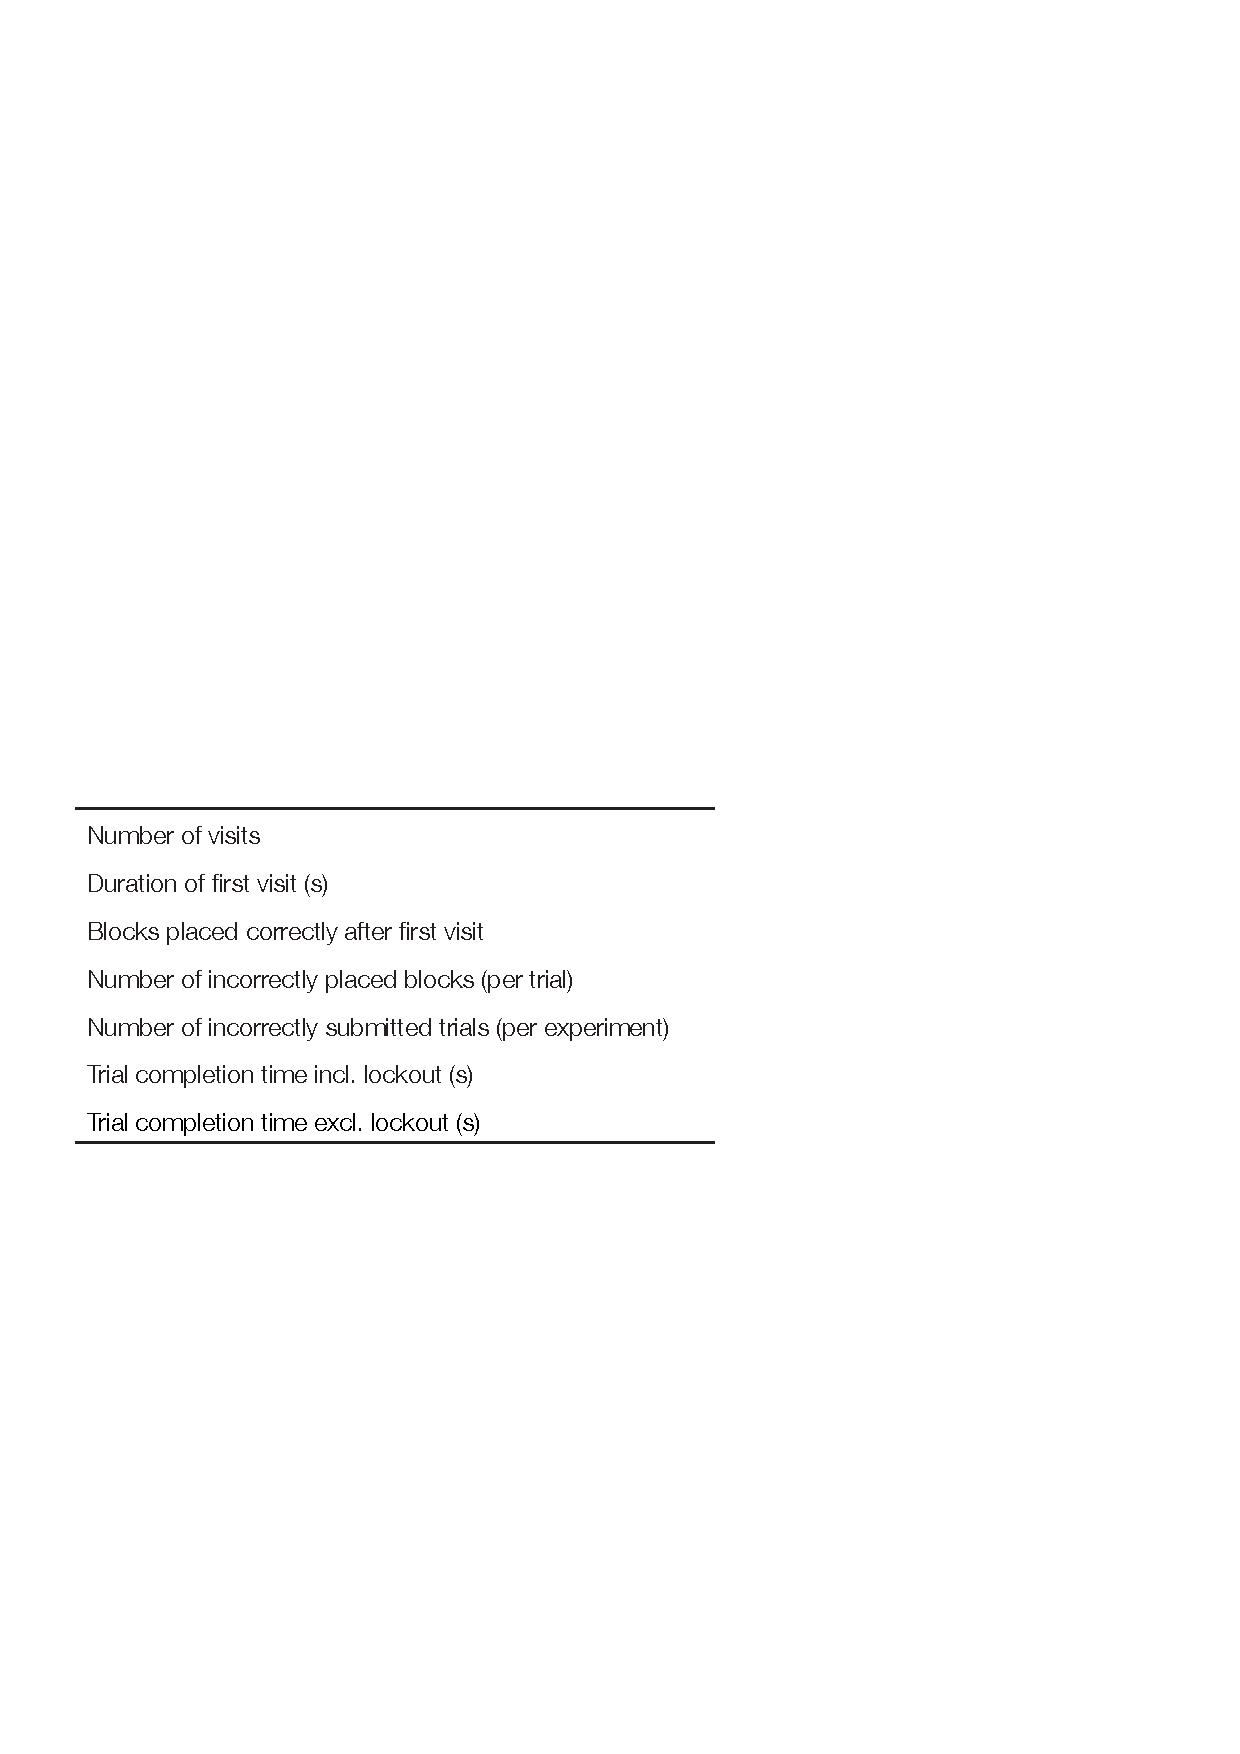
\includegraphics[width=0.6\textwidth]{images/ch34/ch34-3_DVs.pdf}
    \caption[Study 3 dependent variables]{Dependent variables used in the study.}
    \label{table:ch4_dvs}
\end{table}

The number of blocks copied after each visit were measured by using JavaScript, which recorded all drop events of blocks into the output window. The position where it was placed on the 3x3 grid was used to determine whether the block was placed correctly.
The primary focus of the analysis was on the measures of the first visit, as participants do not have any information yet on the target pattern. On subsequent visits, they may already have partial information in their head from previous visits. Therefore, the items copied after the first visit are believed to be the most 'sensitive measure of performance' \citep{Janssen2012}. 

Two measures were used to assess accuracy. Incorrectly placed blocks measured instances where a participant initially placed a block in the incorrect place, but then moved this to the correct place prior to submitting the pattern. Incorrectly submitted trials measured instances where the participant had finished copying a pattern and clicked the Submit button, but the pattern was incorrect.

\subsubsection{Procedure}
Participants were welcomed and briefed about the experiment. It was explained they would be shown nine blocks which were in a certain order, and had to copy this order by moving blocks around. Participants were instructed to complete the task as fast as possible, but it was explained that they were not able to continue until they had copied a pattern correctly. 

After the briefing, participants were asked to read and sign a consent form and were given an information sheet with a summary of the study and the researcher's contact details. In addition to the verbal briefing, the explanation of the study was written out on the computer screen for the participant to read and they were shown an instruction video that showed how the experiment worked. 
The experiment was broken down in two parts, one where they had to copy colours, and one where they had to copy numbers. For each part, they were given two practice trials first to get familiar with the set-up, and to give them a chance to ask questions if anything was unclear. There was an opportunity for the participant to take a break between the two parts. The study took around 20-30 minutes to complete.

\begin{comment}
\subsubsection{Ethical considerations}\label{sec:quanethics}
The study was undertaken with ethical approval from the UCL Research Ethics Committee [Project ID Number UCLIC/1415/001/Staff Brumby/Borghouts]. 
At the start of each study, participants were first briefed verbally about the study. They were asked to read and sign a consent form, and were given an information sheet to keep. This information sheet contained a summary of the study information and the researchers' contact details. It was explained that an eye tracker would record their eye fixations and movements, but that these recordings were anonymous and that they would not be directly identifiable. After participants had completed the first part of the experiment, a prompt appeared on the screen advising them to take a short break. Participants could take a break as long as they wanted and could decide themselves when to continue with the second part of the experiment.

Participants were informed that the data would be used for research purposes only and stored in accordance with the Data Protection Act 1998. They were also informed that their data would be anonymised and when used in a report or academic paper, their data would not be directly identifiable.
\end{comment}

\subsection{Results}
The means and standard deviations of all dependent variables are shown in Table \ref{table:ch4_IACmeans}. Two-way mixed ANOVAs were used to analyse the effect of time cost and block type on the dependent variables. A p-value of 0.05 was used for assessing the significance of all statistical tests. 

\subsubsection{Cleaning the data}
Eight participants were removed from the analysis due to weak eye-tracking calibration. Furthermore, one participant misunderstood the experiment and did not know she was allowed to uncover the mask of the target window more than once. This participant had scores that were more than three times the interquartile range from the rest of the participants' scores on six different variables, so this participant was considered an outlier and removed from the analysis. 

\begin{table}
\centering
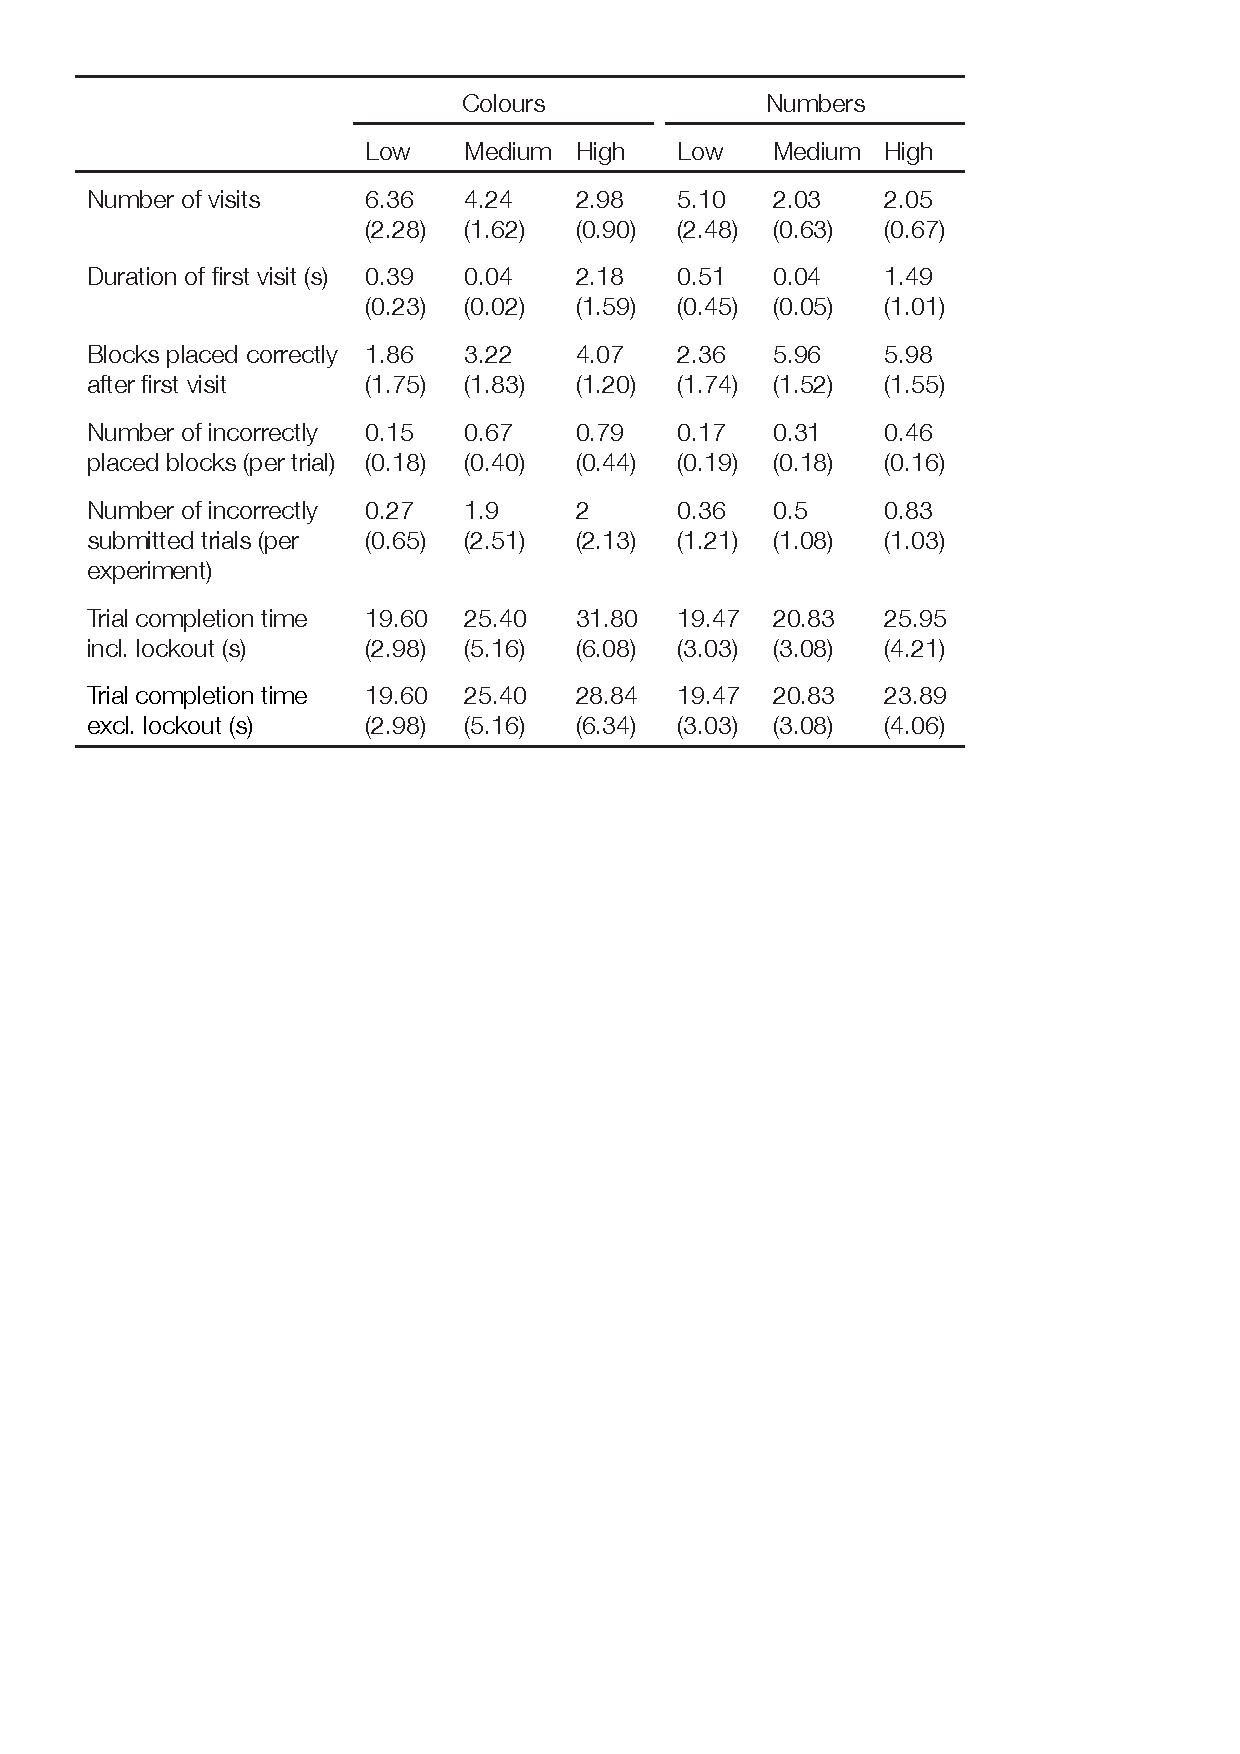
\includegraphics[width=0.8\textwidth]{images/ch34/ch34-3_Means.pdf}
\caption[Study 3 descriptive measures]{The means (and standard deviations) of dependent measures for the different block type and IAC conditions.}
\label{table:ch4_IACmeans}
\end{table}

\subsubsection{Number of visits to the target window}
The number of visits was measured using eye fixations for the Low Cost condition, and the uncovering of the target pattern for the Medium and High Cost conditions. Participants made fewer visits to the target source when they had to copy numbers (M = 3.06, SD = 2.08) than when they had to copy colours (M = 4.49, SD = 2.18), F(1,30) = 41.62, p<.001, $\eta^2$  = .58. Participants also made fewer visits as IAC increased from Low (M = 5.73, SD = 2.41), to Medium (M = 3.13, SD = 1.65), to High (M = 2.51, SD = 0.91), F(2,30) = 15.16, p<.001, $\eta^2$  = .50. To investigate differences between conditions, post-hoc Tukey comparisons were performed. Results showed that participants made significantly fewer visits in the Medium-IAC condition than in the Low-IAC condition, p <.01. However, there was no difference in number of visits between the Medium-IAC and the High-IAC conditions, p=.59. Participants looked at the target window for colours more on every level of IAC, and so there was no significant interaction, F(2,30) = 2.82, p=.08, $\eta^2$  = .16. 

\begin{comment}
\begin{figure}[!ht]
\centering
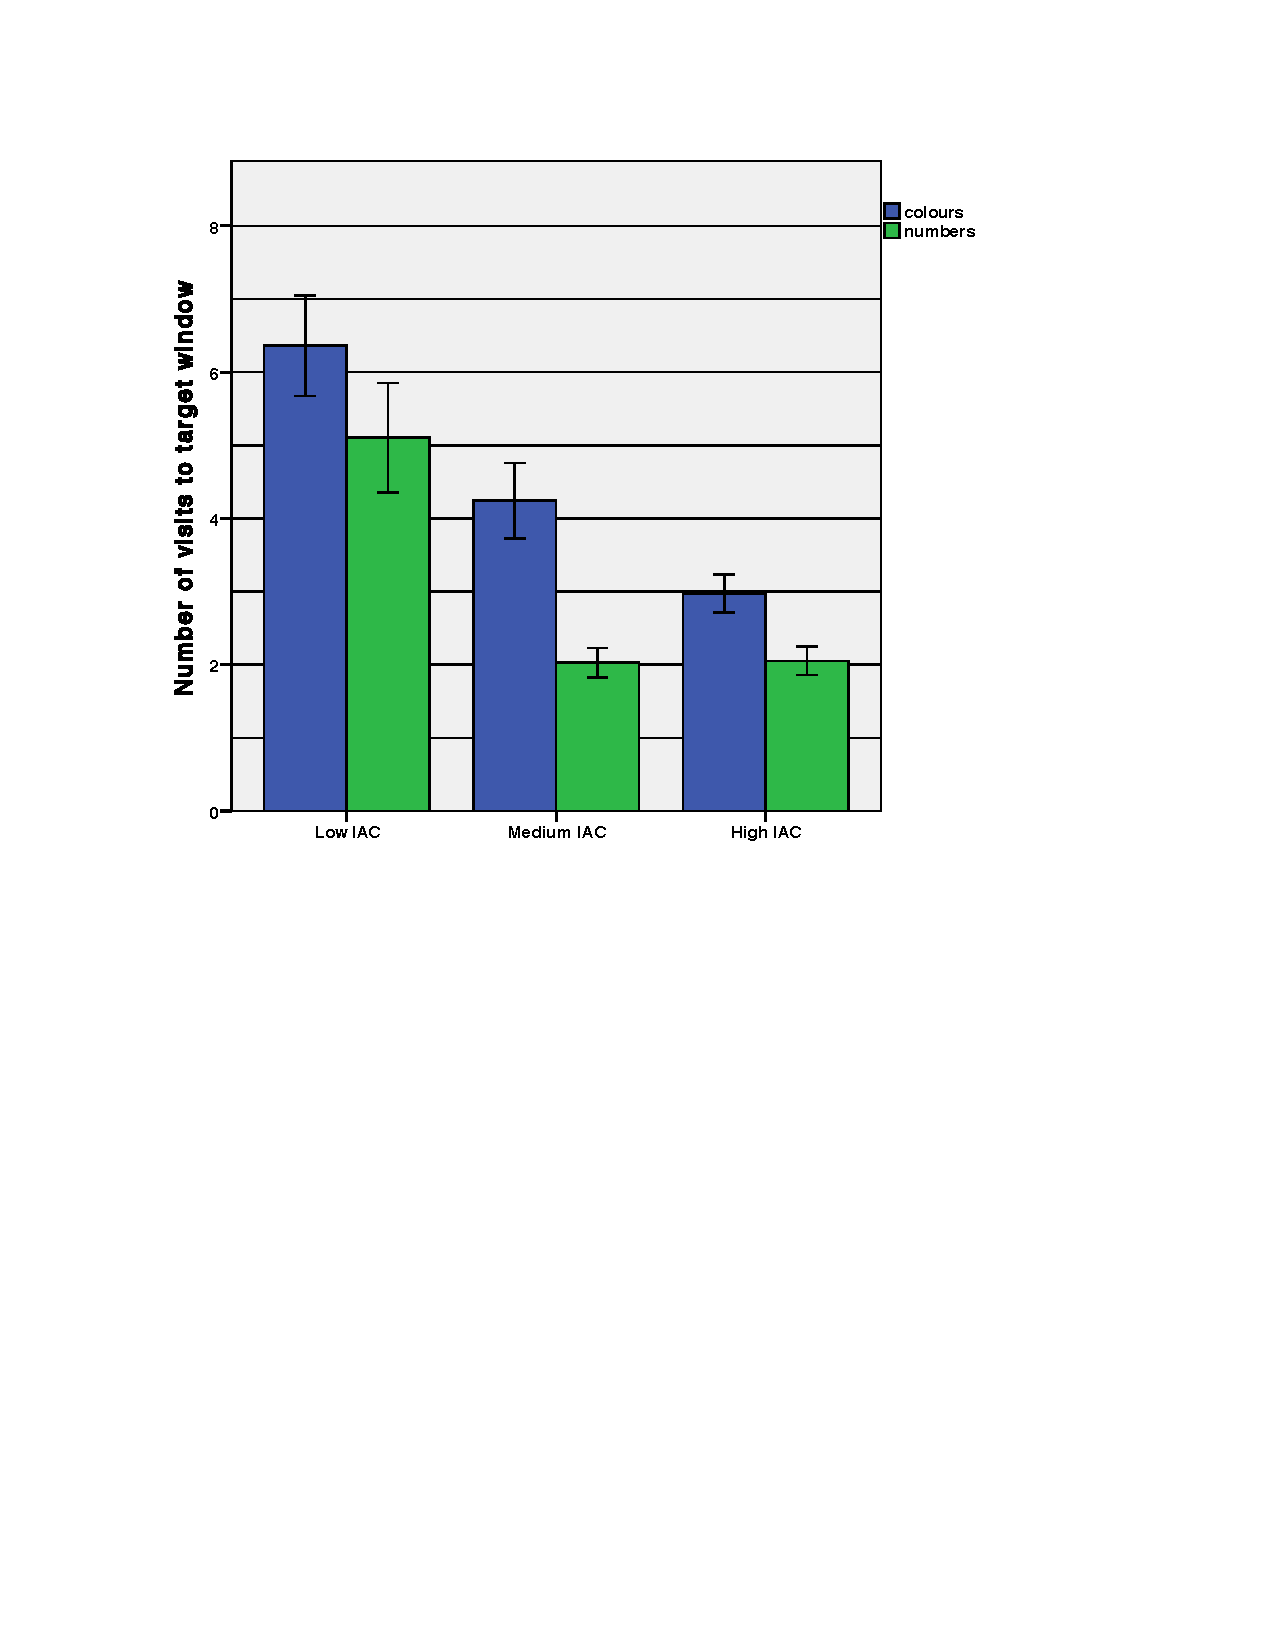
\includegraphics[width=\textwidth]{images/ch34/ch4_noVisits-bargraph.pdf}
\caption[Study 3 number of visits]{The interaction between block type and IAC for number of visits to the target window. The error bars represent $\pm $1 standard error.}
\vspace{-9pt}
\label{fig:ch4_noVisits}
\end{figure}
\end{comment}

\subsubsection{Duration of first visit to target window}
There was no significant main effect of block type on the duration of the first visit, F(1,30) = 3.05, p=.09, $\eta^2$  = .09. There was a significant effect of IAC, F(2,30) = 16.64, p<.001, $\eta^2$  = .53. Participants looked longer at the target source as IAC increased from Low to High. Post-hoc comparisons showed that participants looked longer in the High-IAC condition (M=1.84, SD = 1.35) than in the Low/Medium-IAC conditions, ps <.001. However, there was no difference in duration between the Low-IAC (M = 0.45, SD = 0.46) and the Medium-IAC (M = 0.05, SD = 0.04) conditions, p=.47. There was a significant interaction effect between IAC and block type, F(2,30) = 5.70, p<.01, $\eta^2$  = .28. There were no differences between block types in the Low-IAC condition, t(10) = -1.86, p = .09, nor the Medium-IAC condition, t(9) = -0.29, p = .70. However, in the High-IAC condition, participants looked significantly longer for colours (M = 2.18, SD = 1.59) than numbers (M = 1.49, SD = 1.01), t(11) = 2.76, p = .02.

\begin{comment}
\begin{figure}[!ht]
\centering
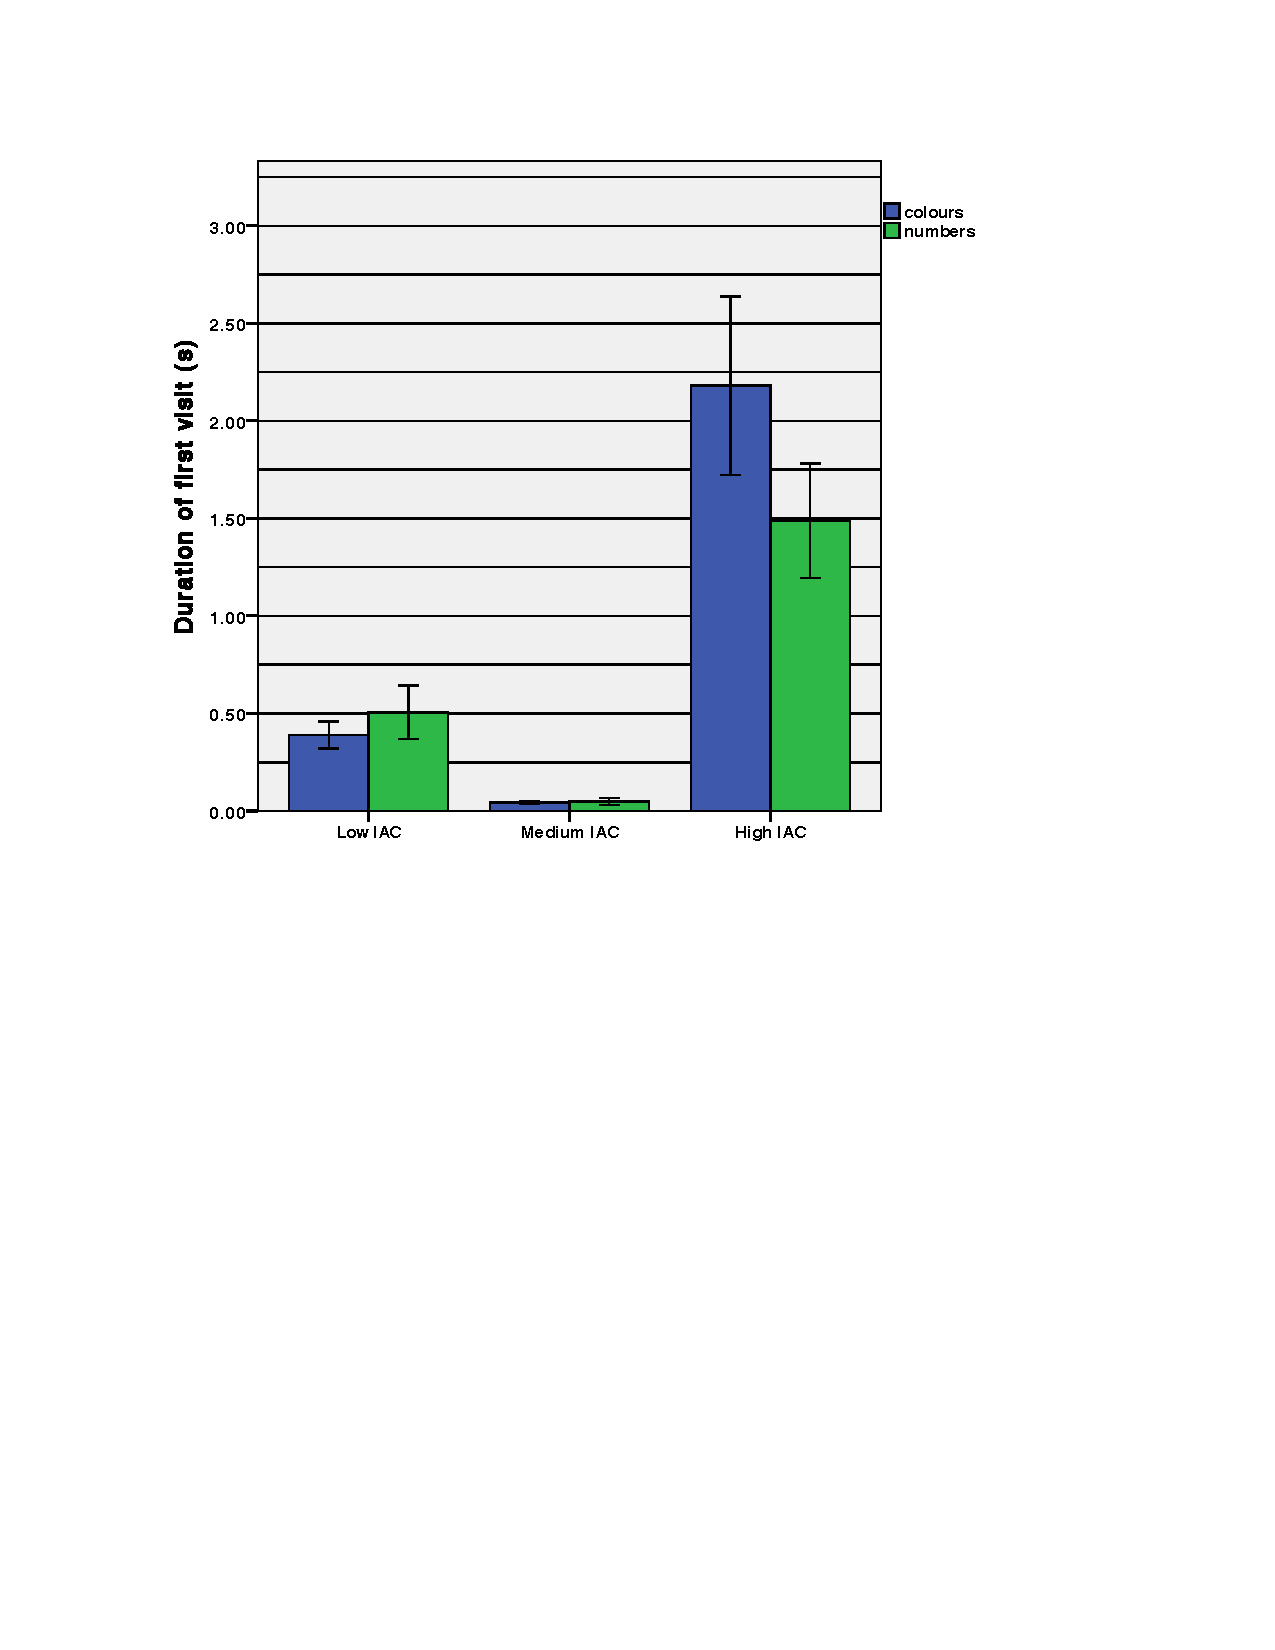
\includegraphics[width=\textwidth]{images/ch34/ch4_firstVisitDuration-bargraph.pdf}
\caption[Study 3 duration of first visit]{The effect of IAC on the duration of the first visit to the target window. The error bars represent $\pm $1 standard error.}
\vspace{-9pt}
\label{fig:ch4_firstVisitDuration}
\end{figure}
\end{comment}

\subsubsection{Blocks placed after first visit}
People placed more blocks correctly after the first visit for numbers (M = 4.77, SD = 2.33) than colours (M = 3.08, SD = 1.81), F(1,30) = 63.86, p<.001, $\eta^2$  = .68. They also placed more blocks as IAC increased, F(2,30) = 12.54, p<.001, $\eta^2$  = .46. Tukey post-hoc comparisons show there was a difference between the Low IAC and Medium/High IAC conditions (ps<.01), but not between Medium and High IAC conditions (p=.77). There was a significant interaction effect between IAC and block type, F(2,30) = 8.96, p<.01, $\eta^2$  = .37. When IAC was Low, the number of blocks that were copied correctly after the first visit did not differ significantly for colours or numbers.

\begin{comment}
\begin{figure}[!ht]
\centering
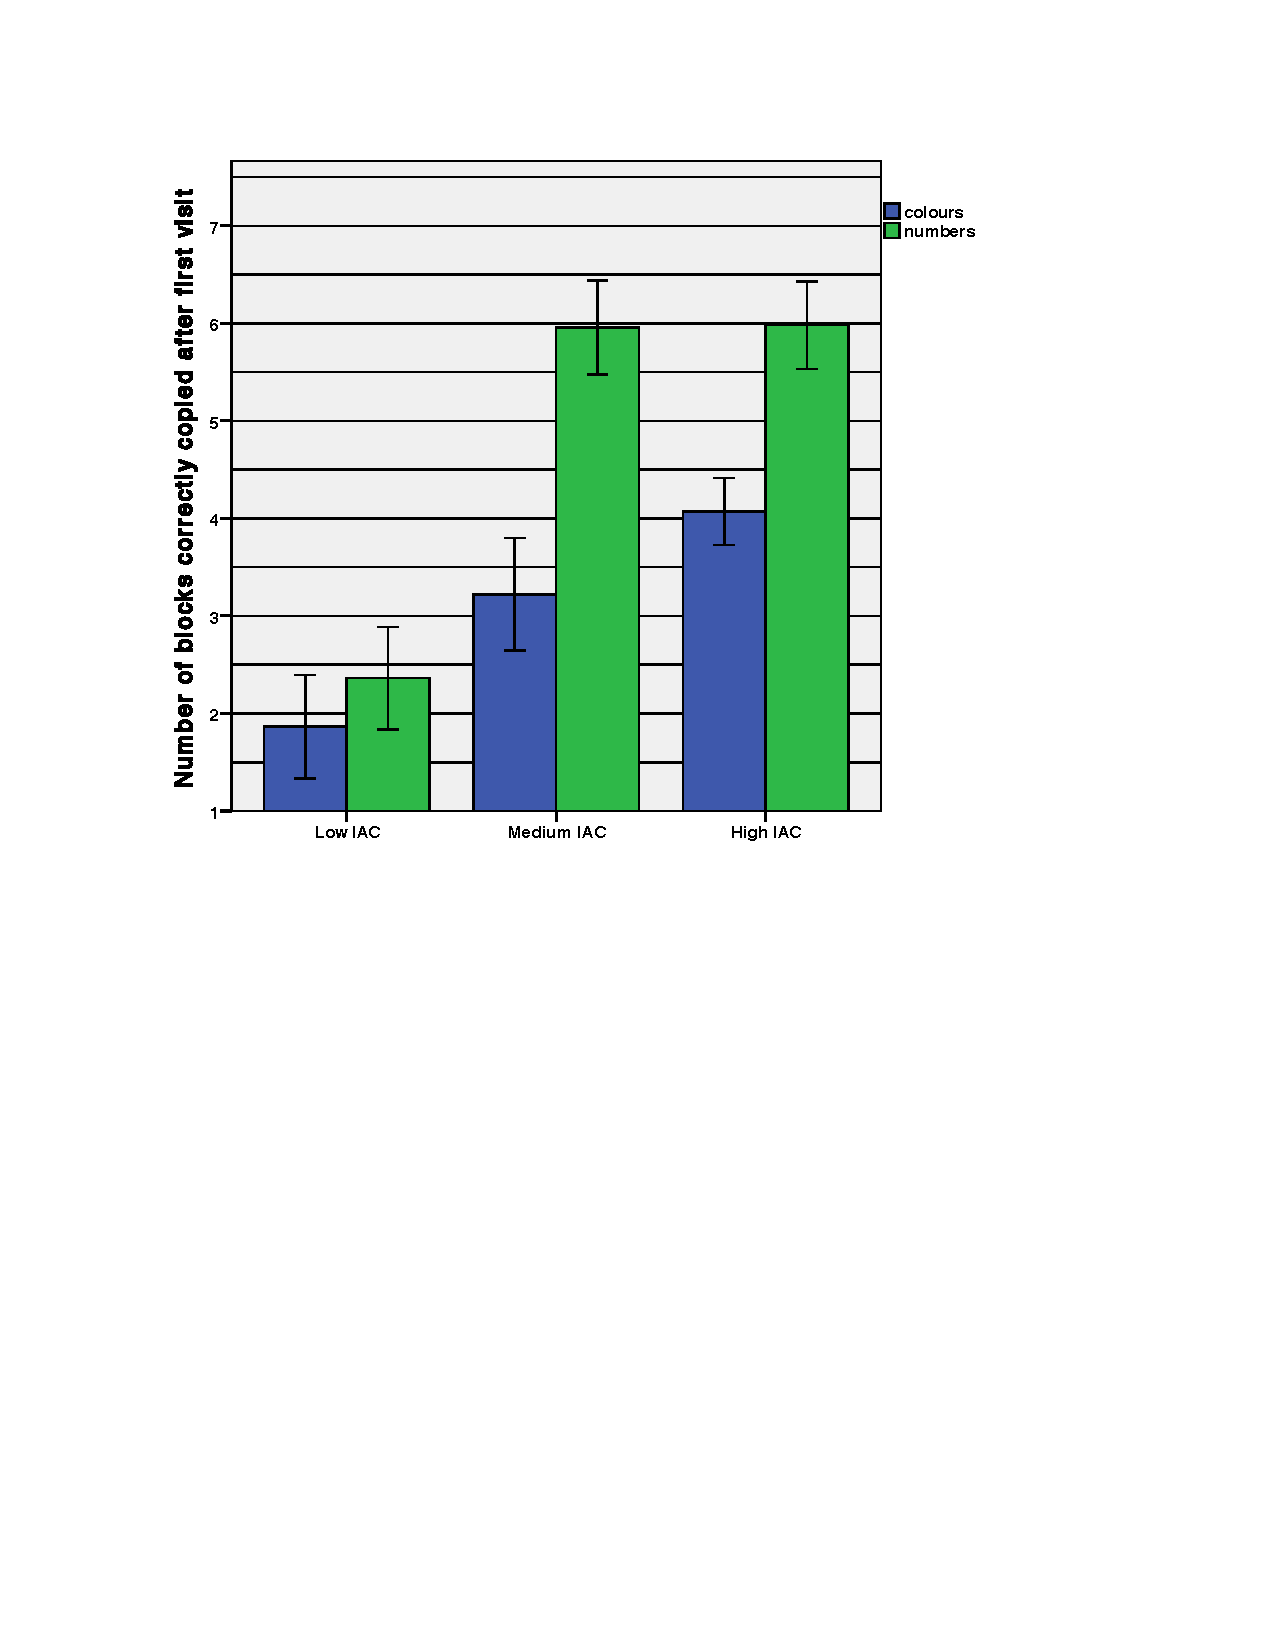
\includegraphics[width=\textwidth]{images/ch34/ch4_firstCorrectBlocks-bargraph.pdf}
\caption[Study 3 number of blocks correctly placed]{The interaction between block type and IAC for number of blocks correctly placed after the first visit to the target window. The error bars represent $\pm $1 standard error.}
\vspace{-9pt}
\label{fig:ch4_firstCorrectBlocks}
\end{figure}
\end{comment}

\subsubsection{Trial completion time}
Two trial completion times are considered here: total completion time including and excluding lockout. 
Looking at the actual completion time, participants took longer to complete a trial when they were copying colours (M = 25.80, SD = 7.06) compared to when copying numbers (M = 22.24, SD = 4.47), F(1,30) = 44.09, p<.001, $\eta^2$ = .60. As IAC increased from Low to Medium to High, participants took longer to complete a trial, IAC, F(2,30) = 15.91, p<.001, $\eta^2$ = .52. Tukey post-hoc comparisons show there was a difference between Low/Medium and High (ps<.01), but not between Low and Medium (p = .12). There was a significant interaction effect between IAC and block type, F(2,30) = 11.05, p<.001, $\eta^2$ = .42. When IAC was Low, completion time did not differ significantly for colours or numbers, but as IAC increased, participants were slower to copy colours.

With the lockout time in the High-IAC condition removed, the same effects were found for block type, F(1,30) = 34.55, p<.001, $\eta^2$ = 0.54, and IAC, F(2,30) = 8.18, p<.01, $\eta^2$ = .35. Tukey post-hoc comparisons show there was still a difference between Low and High (p<.01), but no longer between the Medium IAC and Low IAC or High IAC conditions (ps >.1). There was again a significant interaction effect between IAC and block type, F(2,30) = 8.13, p<.01, $\eta^2$ = .35.

\subsubsection{Number of incorrectly placed blocks}
Participants placed more blocks incorrectly for colours (M = 0.54, SD = 0.45) than numbers (M = 0.32, SD = 0.21), F(1,30) = 10.72, p<.01, $\eta^2$ = .26. %p= 0.003
As IAC increased and participants were keeping more items in memory, they increasingly placed more incorrect blocks, F(2,30) = 14.71, p<.001, $\eta^2$ = .50. Tukey post-hoc comparisons show there was a difference between the Low IAC condition (M = 0.16, SD = 0.18) and Medium/High IAC conditions (ps<.01), but not between the Medium (M = 0.49, SD = 0.35) and High IAC conditions (M = 0.63, SD = 0.36) (p = .30). There was a significant interaction effect between IAC and block type, F(2,30) = 3.36, p<.05, $\eta^2$ = .18. When IAC was Low, the number of blocks that were copied incorrectly did not differ significantly for colours or numbers, but as IAC increased, participants placed more blocks incorrectly for colours.

\subsubsection{Number of incorrectly submitted trials}
The number of trials that were submitted incorrectly was generally low, but participants submitted more incorrect trials for colours (M = 0.1, SD = 0.16) than numbers (M = 0.04, SD = 0.08), F(1,30) = 5.28, p=.03, $\eta^2$ = .15. There was no significant effect of IAC, F(2,30) = 2.70, p=.08, $\eta^2$ = .15, nor any interaction, F(2,30) = 1.65, p=.20, $\eta^2$ = .10.

\subsubsection{Qualitative data}
The screen recordings from the eye-tracker were played back to further investigate people's behaviour. Although this helped understand some behaviour which could not be determined from the quantitative data alone, these observations only serve to explain some of the quantitative measures and are not the main focus of the analysis.

The visit durations in the Medium IAC condition were suspiciously short. Upon replaying the screen recordings, it appeared that participants often accidentally moved their cursor over the grey mask of the target source. This was counted as a visit by the program, even though participants may have not intentionally moved their cursor to this part of the screen to look at the target source. They did not spend a long time looking at the target window, but also did not immediately move blocks either, and sometimes waited multiple seconds before they made a move. 

During the 1-s lockout in the High IAC condition, participants changed their minds about visiting the target window on numerous occasions. They placed their mouse cursor on the mask, but left this field before it was uncovered to move one or more blocks. It could be this decision also occurred in the Medium IAC condition, but as there was no lockout the mask was already uncovered before people made this decision, and would explain the very short visits.

People sometimes placed the blocks as 'placeholders' as shown in Figure \ref{fig:ch4_placeholders}: they placed several blocks outside of the output window next to the position they thought it belonged to, but did not place it there yet. Only after viewing the target again, they placed the blocks in the output window. Looking at quantitative data alone, this type of strategy would be depicted as one long view at the target, after which all blocks were placed in one go. This is true to some extent, but as people could already place the blocks and offload their memory without this being recorded by the program, they only had to check if this position was correct on the subsequent visit, and is different from a strategy where people spent a long time trying to memorise the blocks after which all blocks were placed.

\begin{figure}[t!]
\centering
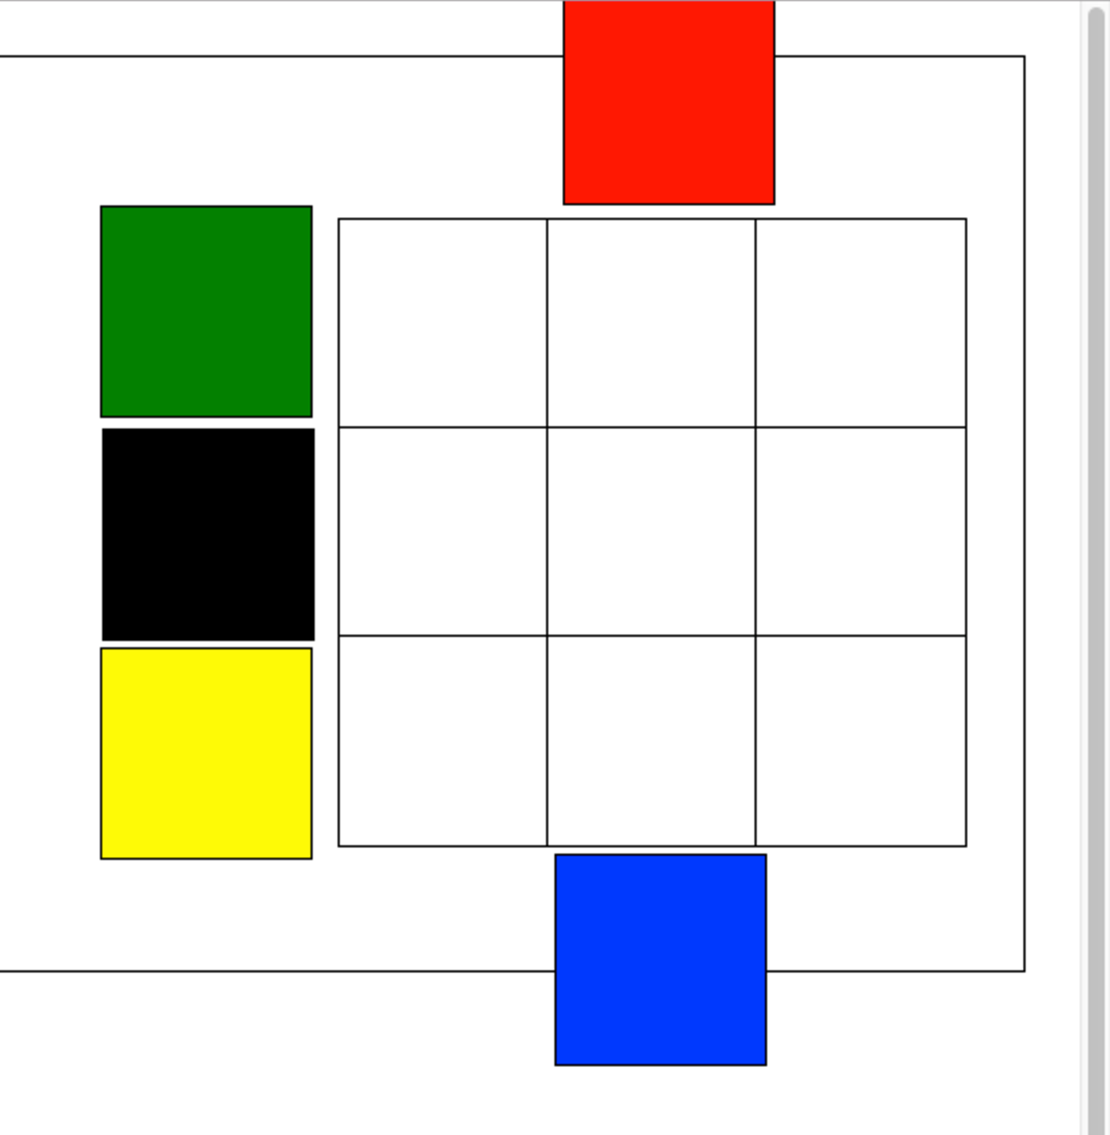
\includegraphics[scale=0.3]{images/ch34/ch4_placeholders.pdf}
\caption[Study 3 placeholders]{Participants placed blocks outside of the output window as `placeholders'.}
\vspace{-9pt}
\label{fig:ch4_placeholders}
\end{figure}

%\newpage

\subsection{Discussion}
The aim of this study was to investigate the effect of time costs on the number and duration of inquiries, and the effect on task performance. The main findings are:

\begin{itemize}
\item
increases in time costs make people adopt memory-intensive strategies
\item
the effect of a memory-intensive strategy on task performance depends on the type of information
\item
the effect of a memory-intensive strategy on task performance depends on the type of task
\end{itemize}

%The study replicated the BWT study to investigate whether the effect of time costs, as found in previous experimental studies, would extend to different types of information. We learn that people try to avoid time costs, and as time costs increase minimise switches to task information, and instead rely on information in their head. The study shows that the type of information matters: contrary to copying colours, when copying numbers this strategy did not increase any errors so may be a safe strategy, although it did not increase people’s performance either. 

%We also learn that the type of task matters: slowing people down, but not realistic. 

%Memory-intensive strategy
The findings support hypotheses H1 and H2: as IAC increased, people switched from a perceptual to a memory-based strategy by making fewer (H1) but longer (H2) visits to the target window. As a result, they placed more blocks immediately after the first visit. This effect of time costs is consistent with prior work \citep{Gray2006, Morgan2009, Waldron2007}, and further confirms that in a controlled setting, people are sensitive to small increases in time costs and try to avoid time costs.

%The effect of time costs on people's strategies is consistent with prior work \citep{Gray2006, Morgan2009, Waldron2007}. As IAC increased, people switched from a perceptual to a memory-based strategy by making fewer but longer visits to the target window and placing more blocks immediately after the first visit. This further confirms that in a controlled setting, people are sensitive to small increases in time costs and try to avoid time costs.

In the Colours condition, a memory-intensive strategy worsened participants' task performance, as they took longer to complete the task and placed more incorrect blocks throughout the trials. In the Numbers condition, a memory-intensive strategy did not increase errors, which shows that the type of information matters when considering whether a memory-intensive strategy is beneficial or not. Numbers were likely easier to memorise, which was demonstrated by the higher number of blocks that were copied after a first visit to the target window: on average, people placed six numbered blocks after a first visit, which is about the number of items people can hold in short-term memory \citep{Miller1956}. In comparison, people only placed on average three coloured blocks after a first visit. Numbers can be rehearsed, and therefore refreshed in working memory, whereas visuo-spatial information such as coloured blocks is more difficult to memorise \citep{Baddeley1974}. 

The findings do not support hypotheses H3 and H4. As IAC increased, a memory-based strategy in the Numbers condition did not make people faster (H3) and they did not make fewer errors (H4). This difference from prior work \citep{Gray2004, Soboczenski2013} could have been due to the nature of the task. In the current study, the error rate was overall low. Upon reflection, the interaction of moving blocks may have made people sufficiently slow to hardly make any errors. In previous studies, people typed in data using a computer keyboard, in which it is more likely to make data entry errors due to slips \citep{Oladimeji2011}.

%Contrary to prior work however \citep{Gray2004, Soboczenski2013}, a memory-based strategy when copying numbers did not make people more efficient or accurate, which could have been due to the nature of the task. The error rate was overall low and upon reflection the interaction of moving blocks may have made people sufficiently slow to hardly make any errors. In previous studies, people typed in data using a computer keyboard, in which it is more likely to make data entry errors due to slips \citep{Oladimeji2011}.
 
 \subsubsection{Limitations}
The study used a similar manipulation of time costs as in previous BWT studies \citep[e.g.][]{Morgan2009, Patrick2014, Waldron2007, Waldron2011}: in the Low Cost condition, the information was permanently visible, and in the Medium and High Cost conditions, the information was covered by a grey mask. Using this manipulation, it was difficult to measure visits to the target window in the same manner for all conditions. For the Low Cost conditions, eye fixations were used, whereas for the Medium and High Cost conditions, uncoverings of the mask were used. 

Measuring visits to the target pattern through eye fixations and mouse movements had a number of limitations.  
%Limitation of eye fixations: you do not know people are actually looking at the screen
First, while eye-tracking measures show how long and how often people are looking at a particular part of the screen, it can not reveal if people are actually perceiving or processing the data that is displayed \citep{Waldron2007}. Second, the results showed unexpectedly short visits for the Medium Cost condition. Playing back the screen recordings revealed that participants often accidentally uncovered the target window when they were moving their computer mouse, and it is therefore unclear if these uncoverings are a reliable measure of actual visits. Lastly, because visits were measured differently across conditions, the results from the Low-IAC condition may not be directly comparable with the Medium-IAC and High-IAC conditions. Therefore, for the next two experiments in this chapter the experimental setup was adapted so that participants had to make a conscious decision to reveal the target information, and were less likely to accidentally access the source when they did not intend to. Furthermore, the same consistent measure was used across conditions (i.e. a mouse click to make a window switch) to study inquiries. 

 %Limitation of uncoverings
% For the Medium and High Cost conditions, an interaction was required and a conscious decision had to be made to reveal the target in these conditions. It would therefore seem likely that uncoverings more reliably measure visits to the target window. However, the uncoverings for the Medium Cost conditions were rather short. Playing back the screen recordings suggests participants often accidentally uncovered the window, and it is therefore less clear if these are a reliable measure of actual visits. In future studies, the setup of the experiment should be designed so that participants make a conscious decision to reveal the target information, but do not accidentally access the source when they do not intend to. In the next two experiments, the same consistent measure is used (i.e. a mouse click to make a window switch) to study inquiries across conditions. 
 
 %Limitation of using different measuremenst 
% Second, visits were measured differently in different conditions, care should be taken to compare results from the Low-IAC condition with the Medium and High-IAC condition. 
 
 \subsection{Conclusion}
The aim of this study was to investigate the effect of time costs on number and duration of inquiries and task performance. The results show that if people retrieve all data from the same source, they will reduce switches between entering and looking up data if the access cost to this source increases. As it took more time to access, offloading behaviour was observed as well, and several participants prepared items they were going to need nearby, but did not use them yet. 

The overall aim of this chapter is to investigate the effect of time costs on inquiry strategies. Study 3 showed that time costs reduce number of switches and increase duration of switches. The task however only involved one source, in contrast with the task studied in Study 1 and 2, where people had to deal with various sources, all with different time costs. While we now have a better understanding of the effect of time costs on number and duration of inquiries, we do not know the effect on the timing of inquiries yet. This will be investigated in the next two studies.

%As a result, people not only have to make decisions on how often they make inquiries to these sources, but also when they interrupt their task to make inquiries.

\section{Study 4: Inquiries to multiple sources}\label{st:Study4}
 
\subsection{Introduction}
%Motivation
Study 3 showed people avoid time costs by making fewer inquiries to an information source. Participants tried to group and memorise as much information, in order to minimise the number of revisits to this source. In the experiment, all information was to be found on a single source. As discussed in Chapter \ref{ch:12}, data entry in office workplaces is often more complex than switching between a task and a single source: information can be spread over various sources with different time costs associated with them. Information can be one click away, or time has to be spent accessing it. What we do not know from Study \hyperref[st:Study3]{3} is how time costs affect how people schedule inquiries to multiple sources, with \textit{different} time costs. Observational findings from Study \hyperref[st:Study2]{2} suggest that inquiries with a high time cost are postponed: participants prepared physical information sources either before starting work or postponed it to access later. Digital information sources however were often accessed during the task, as these were presumed to be quick to retrieve. Furthermore, in prior work \citep{Sohn2008} information access cost was found to be a main factor that determined whether participants looked up information on their mobile phone as soon as they needed it, or whether they postponed to address it later. While these findings demonstrate people take time costs into account when accessing information on physical sources and mobile phones, it is unclear whether participants take time costs of switching windows on a desktop computer into account. Easy switching between windows on conventional desktop computers may give the false impression that information is easy to access \citep{Sellen2003}. 

The aim of Study \hyperref[st:Study4]{4} is to understand the effect of time costs on the timing of inquiries for a data entry task. An experiment was conducted in which participants had to complete a data entry task, and look up the to-be-entered items by switching to two different computer windows. While prior work has demonstrated that various tasks can involve the use of multiple information sources \citep{Cangiano2009, Murphy2016, Su2013}, it has not been measured how people access these sources, and to what extent the time cost to access a source influences these decisions. Based on the postpone strategies observed in Study \hyperref[st:Study2]{2}, the following hypothesis is made:

\begin{itemize}
\item [H1.]
As the experiment progresses and people become aware how costly it is to access certain sources, they will learn to postpone entering High-Cost items, and choose to enter the Low-Cost items first. 
\end{itemize}

Prior work has shown that increased time costs encourage people to learn more efficient strategies, which they then transfer to use in other situations in which time costs are no longer high \citep{OHara1998, Patrick2014, Waldron2007}. For instance, \citet{Patrick2014} conducted an experiment where participants had to complete a Blocks World Task. Some participants had permanent access to the target pattern, whereas other participants had to complete a number of trials first, in which the target pattern was hard to access. People who were exposed to the interface with an increased access cost first adopted a memory-based strategy and retained this strategy, even when they then interacted with an interface with lower access costs. It is therefore expected that once participants learn it is more efficient to group High-Cost items, they may adopt this strategy for Low-Cost items as well:

\begin{itemize}
\item [H2.]

As the experiment progresses, participants in the High-Cost conditions will learn and choose to enter all Low-Cost items in a batch, and then the High-Cost items in a batch, rather than looking up each item one by one.

\end{itemize}

\subsection{Method}
\subsubsection{Participants}
Thirty-three participants (21 female, 12 male) ranging from 18-52 years (M = 26, SD= 8) took part in the experiment. They were recruited from a university subject pool and received $\pounds$4 for their participation.

\subsubsection{Task}
The aim of the study was to study how people address inquiries from multiple sources for a data entry task. There are currently no existing tasks available that are suitable for this purpose: in existing task paradigms, all information is usually located on a single source. For the purpose of this experiment, I therefore created an experimental task. The experimental task was based on an expenses task, a routine data entry task observed in the studies in Chapter \ref{ch:12}. For this task, the user has to complete a number of data entries regarding incurred expenses in order to get the expenses reimbursed. They enter this data into a claim form, which looks similar to a spreadsheet. 

For each trial, participants were presented with a data entry sheet consisting of two expense claims (see Figure \ref{fig:ch34_4-tasklayout}). They had to complete each row by entering a financial amount to specify an expense that was made, and an account code to specify which account to use to reimburse the expense. They retrieved these data items by switching to two other windows. One window contained the amounts (Step 1 in Figure \ref{fig:ch34_4-tasklayout}), and another window contained the account codes (Step 2 in Figure \ref{fig:ch34_4-tasklayout}). The participant could go to a window by clicking on the corresponding name in the horizontal menu at the top of the screen. Only one window could be viewed at a time and covered the full screen. 

\begin{figure}
 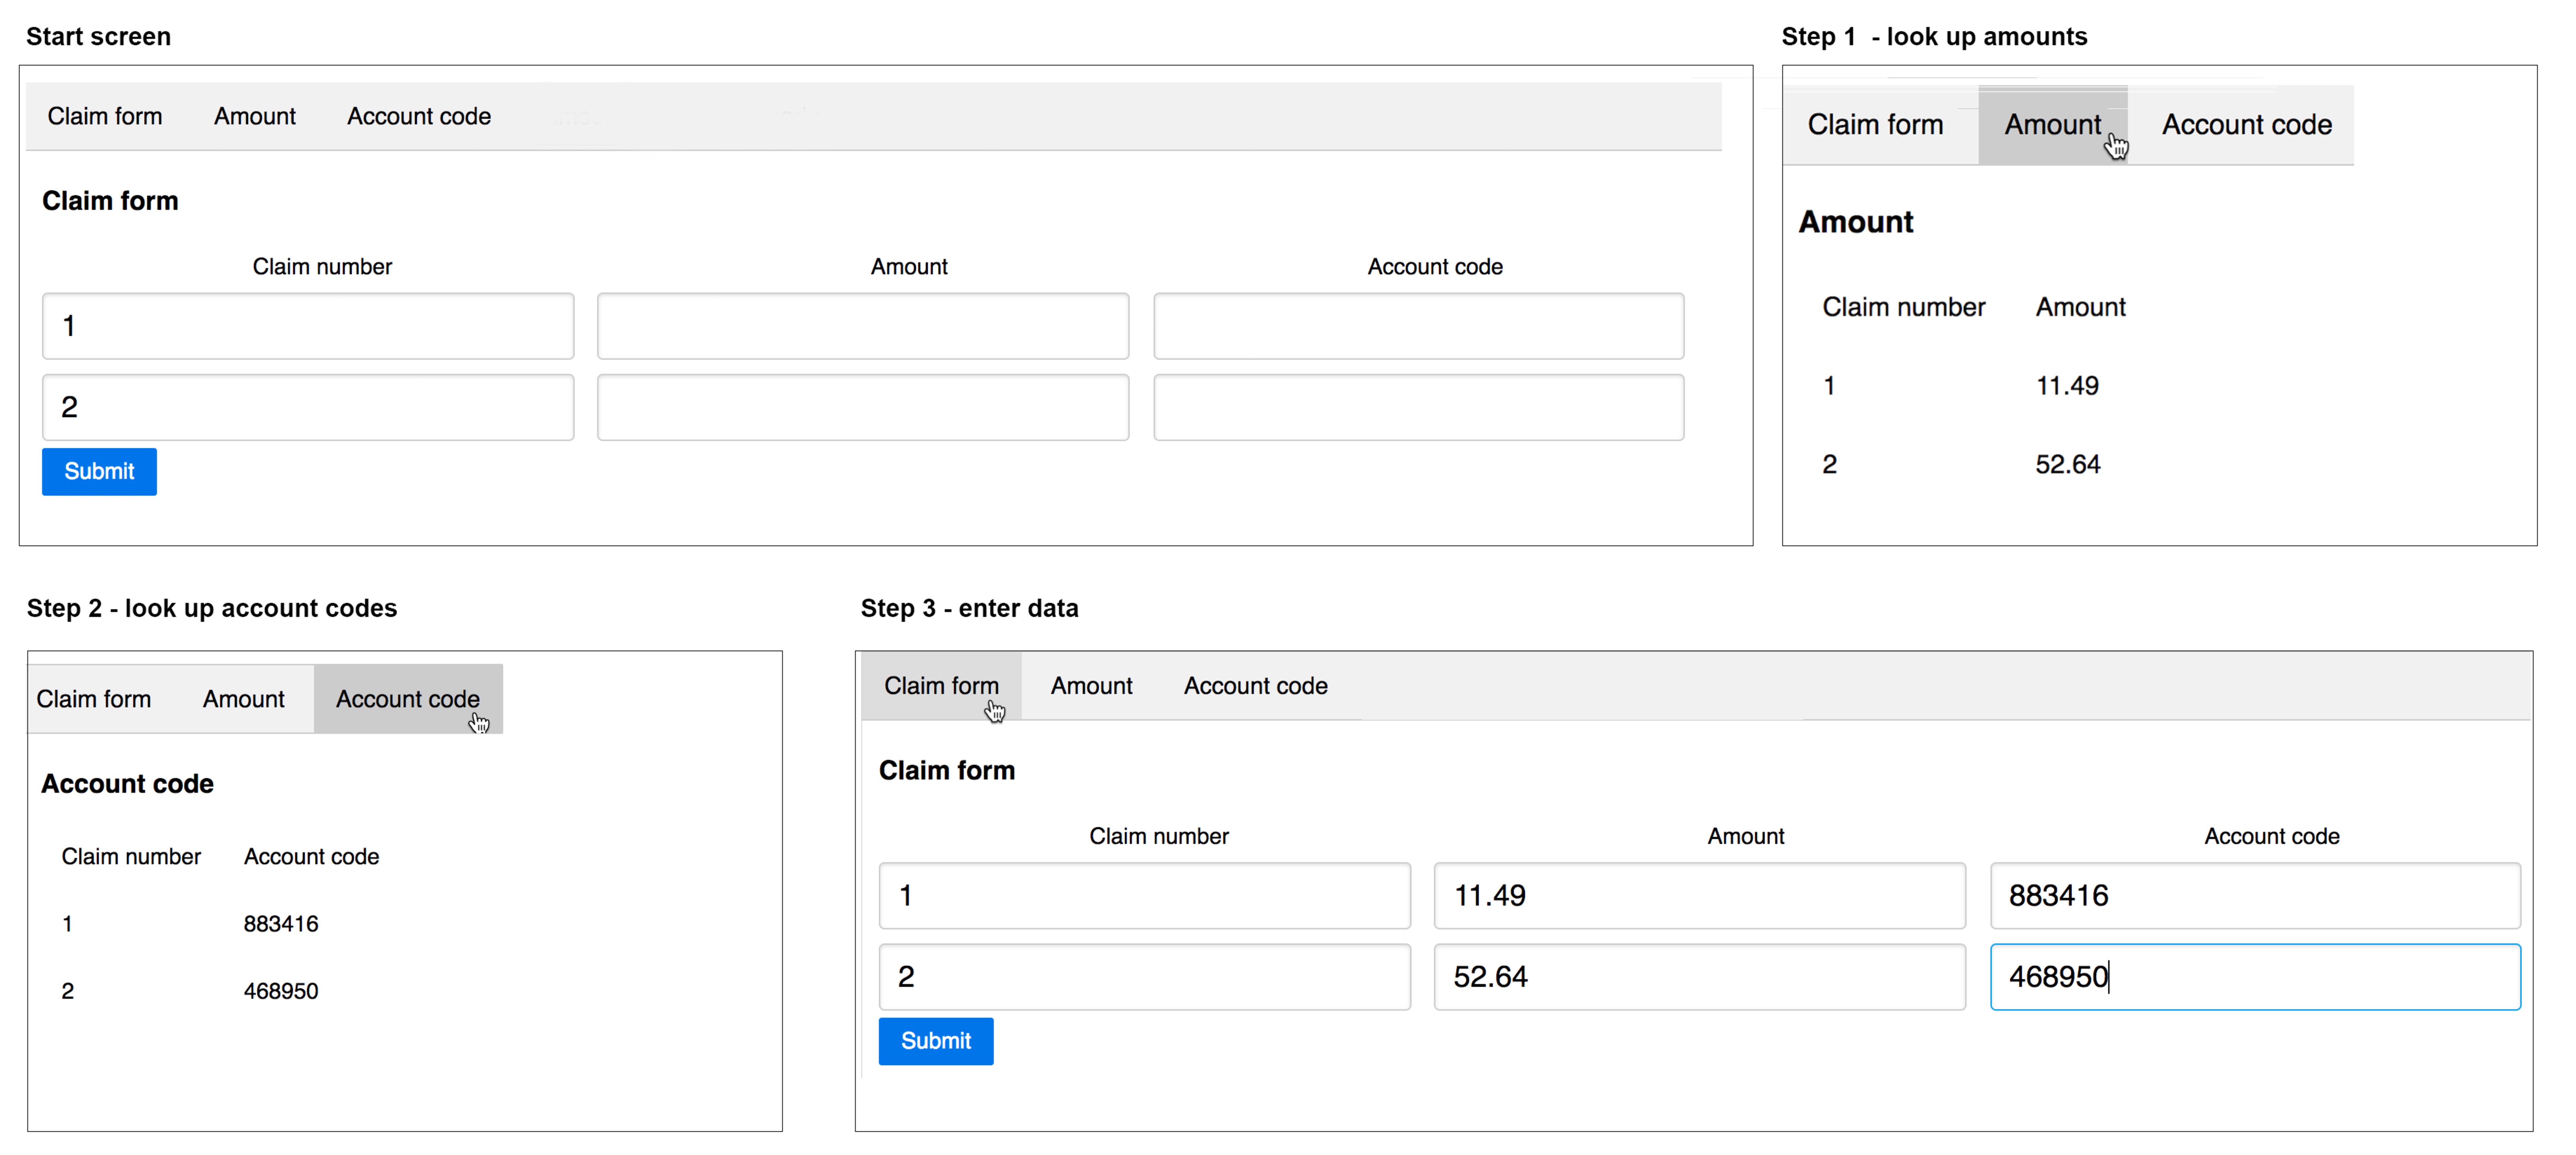
\includegraphics[width=\textwidth]{images/ch34/ch34-4_Tasksequence.pdf}
    \caption[Study 4 data entry task layout]{The data entry task. At the start of each trial, participants were presented with a data entry form with two expense claims, and had to enter four data items in a data entry form. The participant had to switch to an Amounts window (Step 1), and switch back and enter the correct amount in the correct place on the form (Step 2). The participant then had to switch to the Account code window (Step 3) , and switch back and enter the correct amount in the correct place on the form (Step 4). Step 1-4 were repeated for the other items, until all four items had been entered. The participant could switch back and forth between windows as often as needed.}\label{fig:ch34_4-tasklayout}
\end{figure}

\subsubsection{Materials}
The numbers to be entered were made to resemble values that are ecologically relevant to an expenses task. The account codes were similar to codes that are currently used by the universities studied in Chapter \ref{ch:12}, and have a fixed length of six digits (e.g. 654273). The string of digits was random with no particular pattern. Amounts consisted of two digits on the integer part and two digits on the fraction part (e.g. 11.95). 

The experiment was conducted in a maximised web browser on a desktop computer with a 24-inch monitor and a resolution of 2048x1152 pixels. Participants used a computer mouse and number keypad, and it was not possible to copy and paste information. If the participant switched from the data entry form to another window and back, the cursor stayed in the same data entry field. The task interface was developed in HTML, CSS, JavaScript and PHP. All mouse clicks, key presses and timestamps were recorded using JavaScript.

\subsubsection{Design}
A between-participants design was used with one independent variable, the presence or absence of a time cost when switching to one of the information windows. The time cost manipulation in the current study differs from the manipulation used in Study \hyperref[st:Study3]{3}, as the main focus here is to see how people manage inquiries that each have a \textit{different} time cost, as opposed to inquiries that all have the \textit{same} time cost. The manipulation is explained in more detail below. 

In the \textit{Low-Amount, Low-Account} (Low) condition, there were no delays in opening any of the windows. In the \textit{High-Amount, Low-Account} (High-AM) condition, there was a 2-s delay when opening the Amount window, and no delay when opening the Account window. In the \textit{Low-Amount, High-Account} (High-AC) condition, there was no delay when opening the Amount window, and a 2-s delay when opening the Account window. There were no delays in opening the data entry form in any of the conditions.

The Low condition was added as a control condition to understand strategies in a situation where all inquiries had the same time costs, and compare whether these differed from strategies in a High-Cost condition. A High-Cost condition only had a delay on one of the two windows, so that people were presented with both a low and high time cost. This manipulation enabled me to test the hypothesis that people postpone entering High-Cost items in a situation when they can enter Low-Cost items first. Furthermore, there were two high cost conditions, because there were two types of data to be entered (an amount and account code). To know whether any measured differences in inquiry strategies were due to time costs associated with opening a window, rather than the type of data item or the order in which the items were presented, there was one high cost condition where there was a high time cost to access amounts (and a low time cost to access account codes), and another high cost condition where there was a high time cost to access account codes (and a low time cost to access amounts). To simplify notation, from this point onwards these two different High-Cost conditions will be referred to as the High-AM condition and High-AC condition, respectively. 

%An additional condition where all windows had a high time cost is not included in the study, because the interest was not so much on how people access inquiries with the same time cost (regardless of whether it is low or high)

%The main interest of the study was to see how people prioritised inquiries with different time costs. 

%A between-participants design was used with one independent variable, the presence or absence of a time cost when switching to one of the information windows. In the Control condition, there were no costs in switching between any of the windows. In the High-Amount condition, there was a 2-s delay when opening the Amount window, and in the High-Account condition there was a 2-s delay when opening the Account window. There were no delays in switching back to the data entry form in any of the conditions. 

To investigate the timing of inquiries, the order in which participants entered the data items was analysed. On a trial-by-trial basis, the main dependent variable was whether people interleaved between expenses or not: did participants enter the data items in sequential order (i.e. enter one expense first, and then the second expense), or did they interleave between the two expenses to enter items from the same source first (i.e. enter all amounts first, and then all account codes)? Two values had to be entered for each expense: an amount and an account code. If participants entered the amount and account code of one expense before entering the other expense, this was considered a sequential order. If participants entered amounts of each expense first, followed by entering the account codes or vice versa, this was considered interleaving. All window switches and key presses were recorded to determine in which order data was entered. Window switches were recorded to capture the number and duration of switches to information windows. Other dependent variables were trial completion time and data entry error rate. In addition, the type of errors was analysed. 

\subsubsection{Procedure}
The experiment took place in a closed quiet room. It was explained to participants that the task involved entering expenses, and that for each trial they had to enter two expenses. They were not instructed to use a particular strategy, but it was explained it was important to complete all data entry fields before proceeding to the next trial, as they could not return as soon as they had pressed 'Submit'. There were no restrictions in the number or duration of times they could switch between windows, or the order in which they completed the trial. One trial consisted of two expenses, i.e. four data entries. Participants first completed two practice trials to familiarise themselves with the task, and were free to ask any questions; data from these trials were not included in the analysis. After that, the experimental session consisted of 50 trials, divided into 5 blocks of 10 trials. After each block, there was an opportunity for the participant to take a short break. A prompt appeared on the computer screen, and the recording time was paused. Participants could carry on with the experiment by pressing a button on the screen. For each block, a set of 20 different amounts and 20 different account codes were used. These sets were re-used for every block, so in total, each number was presented five times throughout a session. The experiment took approximately 30 minutes.

\subsubsection{Pilot study}
Because the task was newly created for the study and had not been used in previous studies before, two pilot studies were conducted with colleagues to test the task as well as experimental design. The pilot studies were also intended to see if the length of the experiment was long enough for participants to learn and develop strategies, but not too long and tiring to complete.

During the pilot studies, there was a scheduled break after every 5 trials. Both participants mentioned the break prompts happened too frequently, and experienced them as disruptive. They did not find the experiment too long. One participant could not remember which computer windows had an increased time cost. As a result, he did not adapt his strategies according to anticipated time costs and kept entering the data items row by row. The second participant mentioned that the increased time costs definitely made her more careful in checking the numbers were correct. The participants were aware some of the numbers occurred more than once, but the numbers did not occur often enough to be able to memorise them. 

For the main experiments, the breaks were reduced to happen after every 10 trials. In addition, the names of information windows with an increased time cost were underlined in the horizontal menu. This visual feature was added to help participants see more easily which windows had a delay.

\subsubsection{Data analysis of task strategies}
A bottom-up approach was taken to group and analyse people's data entry strategies. For the first iteration of analysis, each trial was grouped into one of two categories: a sequential or interleaving category. If participants first entered the amount and account code of one expense before entering the other expense, this trial was grouped in the sequential category. If participants entered amounts of each expense first, and then entered account codes, or the other way around, this trial was grouped in the interleaving category. On a small subset of trials (<1\%) neither of these strategies was chosen: for example, participants first entered the amount of one expense, followed by the account code of the second expense. These trials were also grouped in the interleaving category, as participants switched to entering the second expense before completing the first expense.

Mouse clicks to switch between windows were used to code the order of people's actions, and get insight into the order in which people visited and entered data items. During the second iteration of analysis, for each trial the order of actions was considered and the trial was either grouped under a new strategy group for this order, or the trial was grouped under an existing strategy group. The most common order of actions is shown in Figure \ref{fig:ch34_4-groupstr}.

\subsection{Results}
Table \ref{tbl:ch34_4-means} summarises the results of the dependent measures for the three conditions. The distribution of the interleaving rate, number and duration of visits, and the error rate were not normally distributed, so non-parametric Kruskal-Wallis tests were used to analyse effects of time costs on these dependent variables. 
A Shapiro-Wilk test suggested that the trial completion times did follow a normal distribution, \textit{W} = 0.95, \textit{p} = .10, so a one-way ANOVA was used to analyse the effect on trial times. A p-value of 0.05 was used for assessing the significance of all statistical tests. 

\begin{table}
 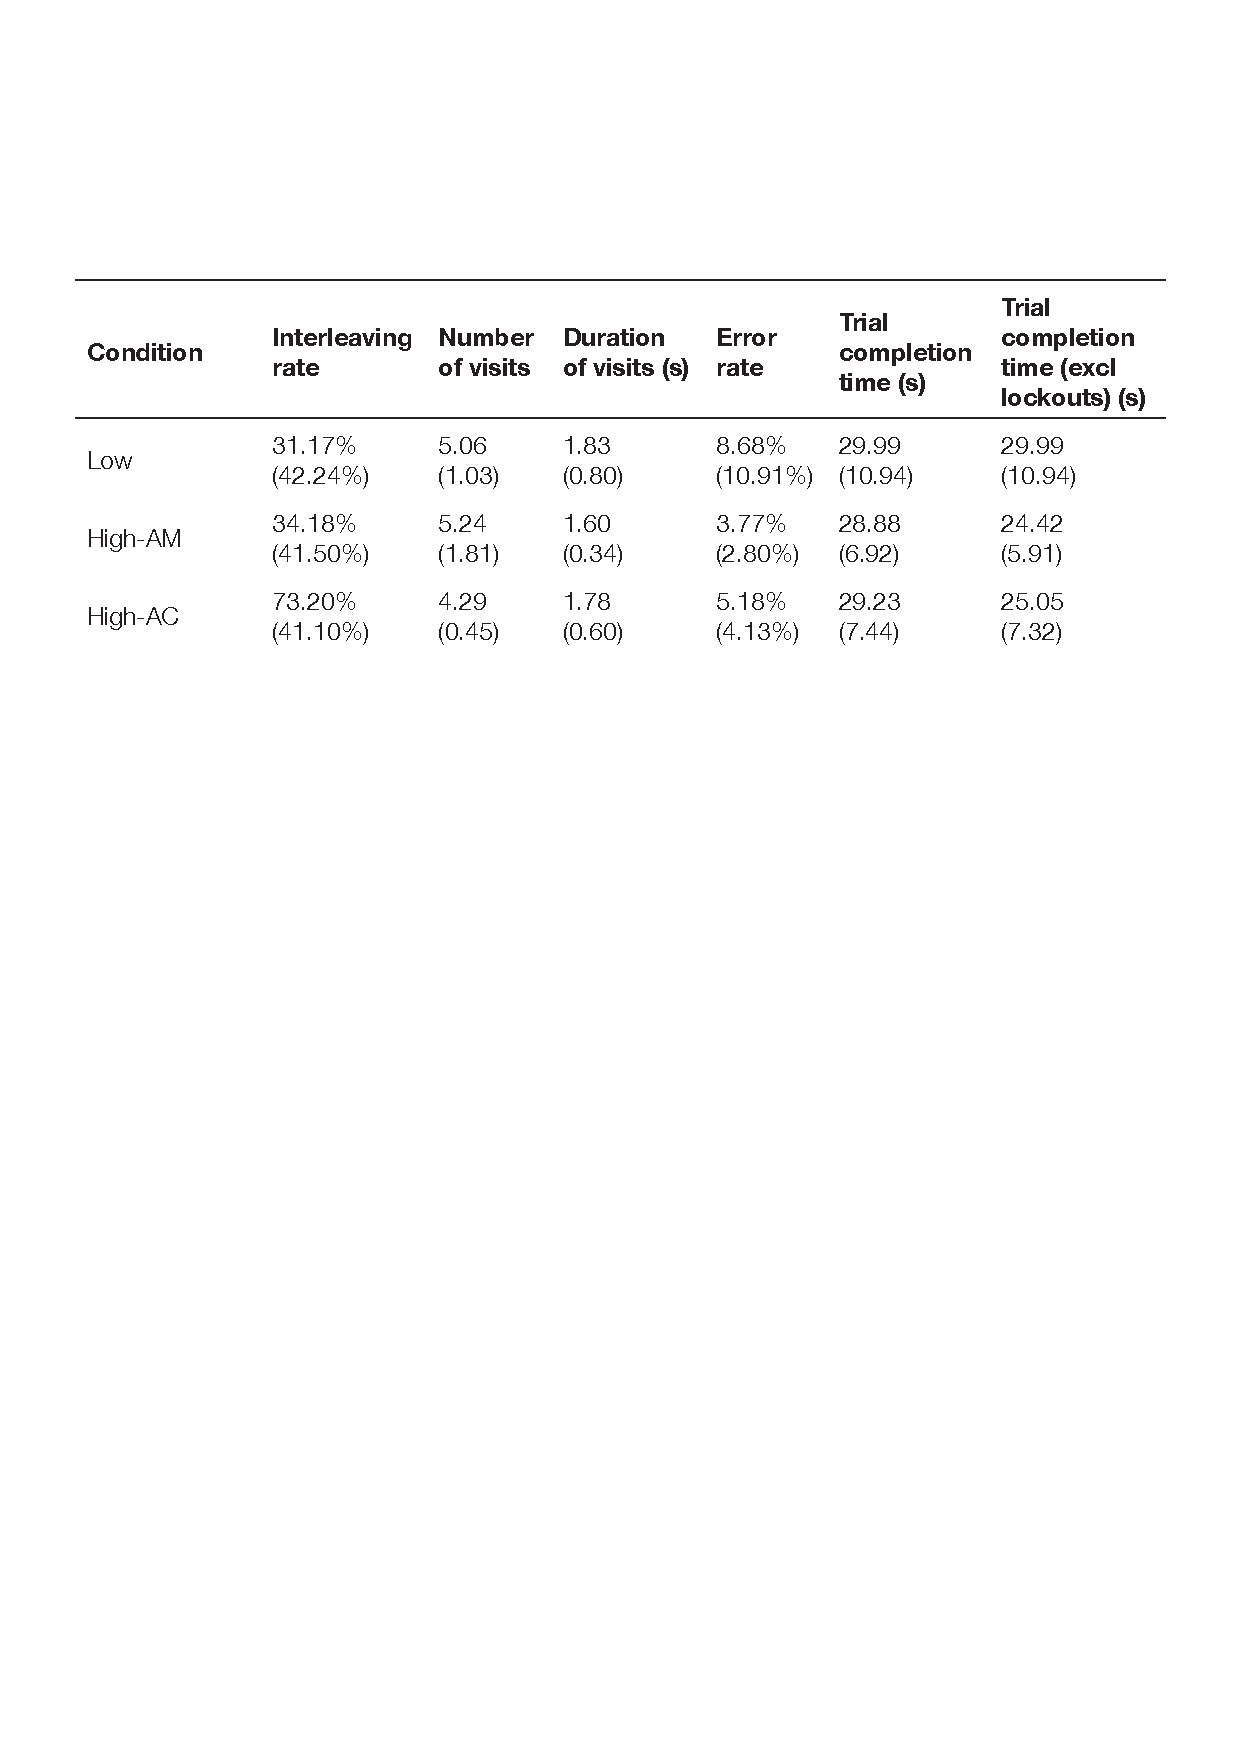
\includegraphics[width=\textwidth]{images/ch34/ch34-4_means.pdf}
\caption[Study 4 means and SDs of dependent measures]{The means (and standard deviations) of all dependent measures for each condition. The rates are calculated by dividing the number of occurrences to the number of opportunities, e.g. an interleaving rate of 50 percent means that on average, a participant interleaved on 50 percent of the trials. In the High-AM condition, there was a delay when opening the Amounts window, and in the High-AC condition, there was a delay when opening the Account window.}
\label{tbl:ch34_4-means}
\end{table}

\subsubsection{Interleaving strategies}
A trial was labelled as 'interleaving' if the participant started entering one expense but interleaved to the other expense before completing the first one. The interleaving rate for each condition was calculated by dividing the number of trials where people interleaved by the number of total trials.  

Across conditions, most participants were consistent in their strategy choice, and either interleaved between expenses on almost no (0\%) or all (100\%) trials. Because the data was centered around these extreme values, for the interleaving rate the medians are reported in addition to the means, as the medians are more representative of the central tendency of the data.

%There was a significant difference between conditions, $\chi^2$(2) = 6.81, \textit{p} = 0.03, with a mean interleaving rate of 73.2\% (Mdn = 96\%) in the High-AC condition, 34.18\% (Mdn = 12\%) for the High-AM condition, and 31.17\% (Mdn = 6\%) for the Low condition. The boxplots in Figure \ref{fig:ch34_4-boxplots} show the variability of interleaving rates across conditions. 

Participants interleaved most often between expenses in the High-AC condition (\textit{M} = 73.20\%, \textit{SD} = 41.10\%), compared to the Low (\textit{M} = 31.17\%, \textit{SD} = 42.24\%) and High-AM (\textit{M} = 34.18\%, \textit{SD} = 41.5\% ) conditions, $\chi^2$(2) = 6.81, \textit{p} = .03. A post-hoc Dunn's test showed there was a difference between the High-AC condition and the Low (\textit{p} = .02) and the High-AM (\textit{p} = .03) conditions, but not between the Low and High-AM conditions (\textit{p} = .90). The median interleaving rate was 6\% for the Low condition, 12\% for the High-AM condition, and 96\% for the High-AC condition. The boxplots in Figure \ref{fig:ch34_4-boxplots} show the variability of interleaving rates across conditions. 

\begin{figure}
 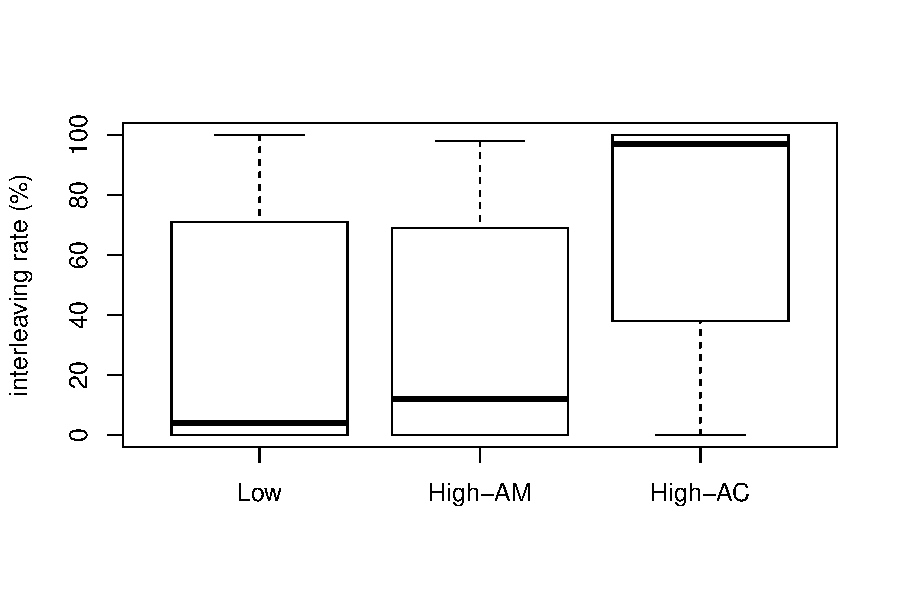
\includegraphics[width=0.6\textwidth]{images/ch34/ch4_4-boxplot.pdf}
\caption[Study 4 boxplot of interleaving rates]{Boxplot of interleaving rates in each condition.}
\label{fig:ch34_4-boxplots}
\end{figure}

Figure \ref{fig:ch34_4-linechart} shows the distribution of interleaving rates for each condition. The lines all have peaks at the left and right end, indicating the interleaving rate was predominantly 0\% or 100\% in each condition. Graphs of each individual participant are included in Appendix \ref{ch:S4_PartPlots}, which shows per trial whether a participant interleaved or not. These graphs further illustrate that participants often used the same strategy throughout the experiment.

\begin{figure}
 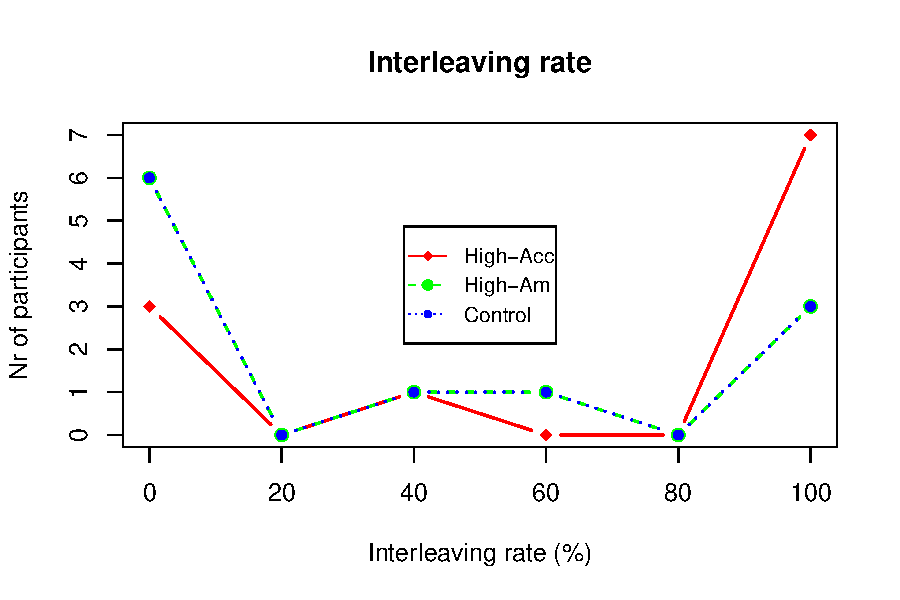
\includegraphics[width=\textwidth]{images/ch34/ch34-4_linechart.pdf}
\caption[Study 4 frequency of interleaving rates]{Line graph showing the frequency of interleaving rates for each condition; the lines of the Low and High-AM condition overlap and follow the same trend. As can be seen, all three lines have two peaks at 0 and 100, which means that most participants interleaved on 0\% or 100\% of all trials.}
\label{fig:ch34_4-linechart}
\end{figure}

\subsubsection{Number and duration of visits}
There was no difference in the number of visits, $\chi^2$(2) = 2.90, \textit{p} = .23. On average, participants made 4 visits per trial (i.e. one visit per data entry). Participants visited an information page for 1.8 seconds on average, and there was no significant difference in duration of visits between conditions, $\chi^2$(2) = 0.30, \textit{p} = .80. 

\subsubsection{Most common order of actions}\label{sec:ch34-StrategyFreq}
To get a better insight in the specific order in which participants viewed and entered items, the trials were grouped based on the order of actions. There were six different possible actions: viewing the amounts window (V-Am), viewing the account codes window (V-Acc), entering the first amount (E-Am1), entering the second amount (E-Am2), entering the first account code (E-Acc1), and entering the second account code (E-Acc2). This iteration of grouping the trials resulted in 12 different strategy groups in total, with the majority of trials (92\%) grouped in the same four groups, which are shown in Figure \ref{fig:ch34_4-groupstr}. In the Low and High-AM conditions, the most common strategy was strategy (a): participants first viewed the Amounts window and entered the amount of the first expense, and then viewed the Account code window and entered the account code of the first expense, before they visited the Amounts window again to enter the amount of the second expense, and view the Account code window to enter the account code of the second expense. Strategy a is also the strategy used in Figure \ref{fig:ch34_4-tasklayout} to illustrate what the task steps in the task interface look like.

In the High-AC condition, participants predominantly used Strategy (c): they first switched to the Amount window, which had no delay, and entered the amount of the first expense in the data entry form, after which they switched to the Amount window again to view and enter the amount of the second expense. After entering the amounts, they viewed and entered the account codes one-by-one.

Table \ref{tbl:ch34_4-groupstr} shows the frequency with which these strategies were chosen per condition. The most common strategy for each condition are highlighted in bold. The table also shows that even though Strategy (a) and (c) were the most commonly observed strategies, these only accounted for about half of the trials: on the other  trials, participants tried out other strategies.  

%For example, the first strategy (a) shows a strategy where participants started a trial by visiting the Amounts window (Am), and then visiting the Accounts window (Acc). They then entered the account code (Acc1) and the amount (Am1) of the first expense. They then visited the Amounts window again, and entered the amount of the second expense (Am2), and then visited the Accounts window again and entered the account code of the second expense (Acc2). Table \ref{tbl:ch34_4-groupstr} shows the frequency with which these strategies were chosen per condition.

%In the High-Account condition, participants predominantly switched to the page with the Amounts first, which had no delay, and entered these into the data entry form. In the other two conditions, participants mostly entered an amount and account code of the first expense first, and then entered the amount and account code of the second row.

\begin{figure}[!ht]
  \centering
    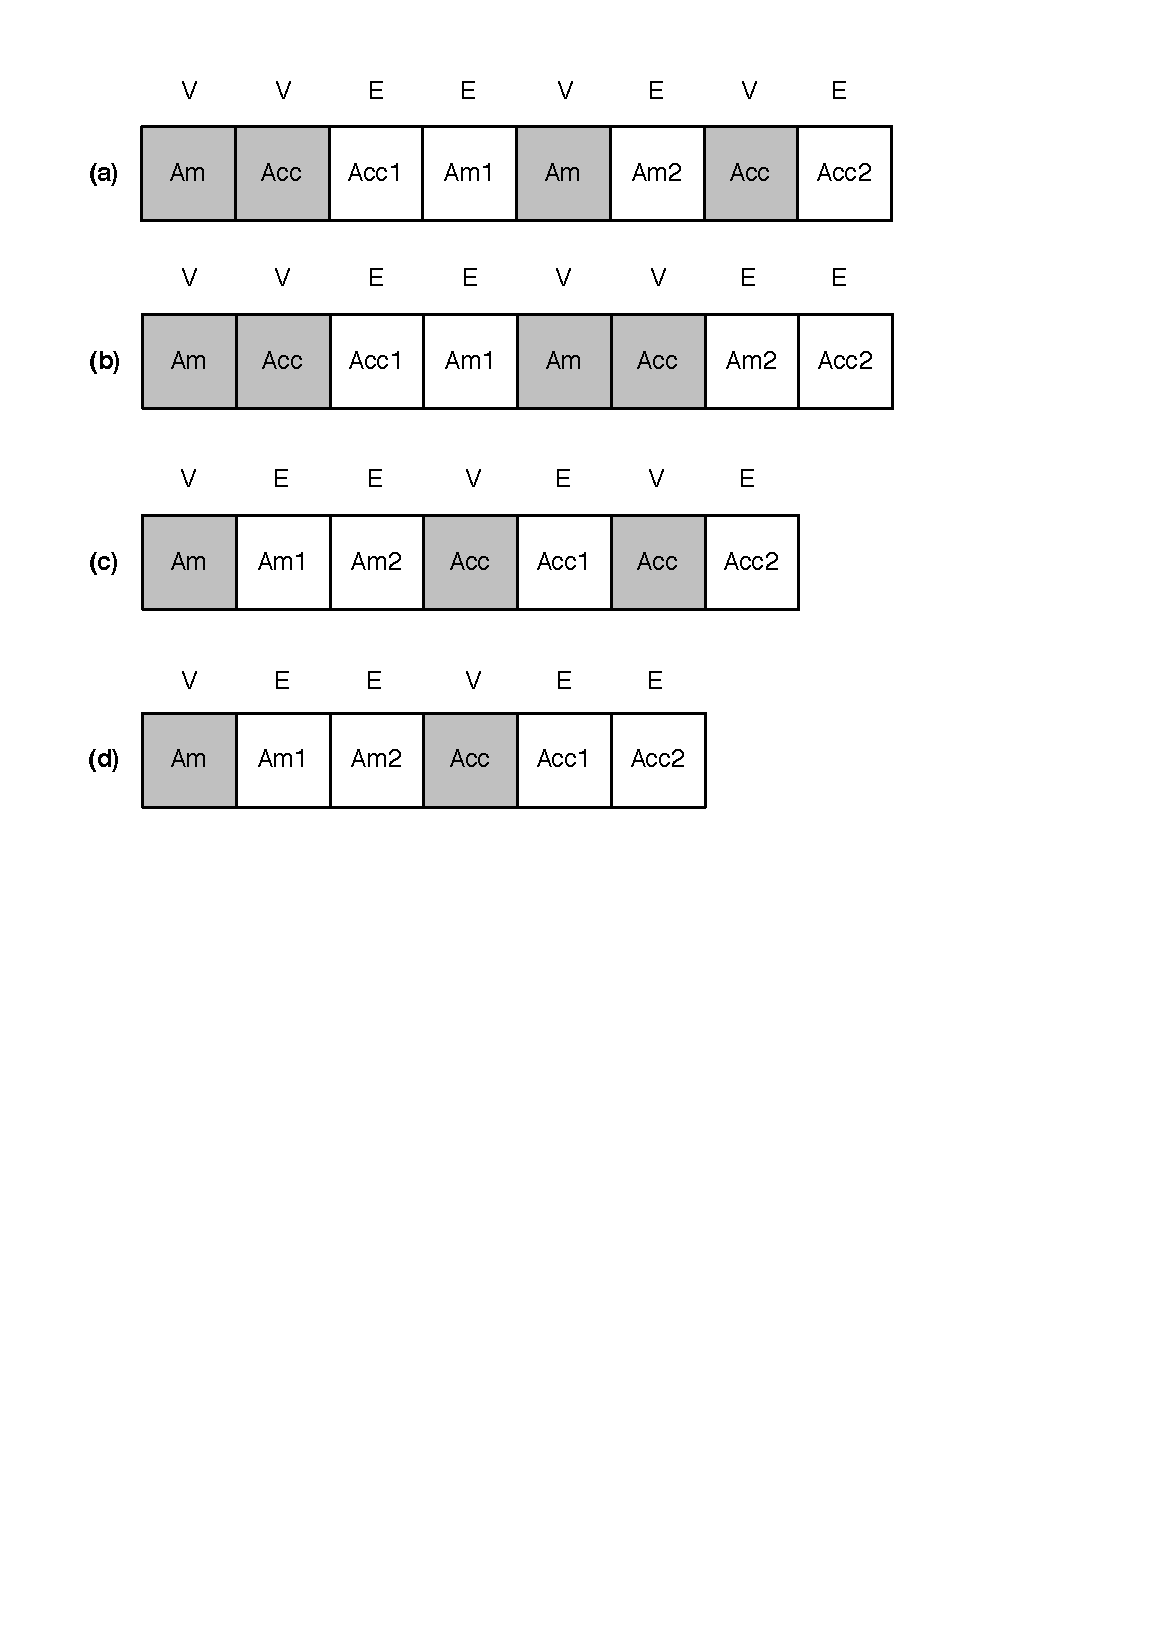
\includegraphics[width=0.5\textwidth]{images/ch34/ch34-4_OrderStrategies.pdf}
      \caption[Study 4 most common order of actions]{The sequence of the most common order of actions. V = visit to an information window, E = entry of a data item. For example, in Strategy (a) a participant first visited the Amounts window, and entered the Amount of the first expense, then visited the Account code window and entered the Account code of the first expense. He/she then viewed the Amounts window again and entered the Amount of the second expense, and then viewed the Accounts window and entered the second expense.}
          \label{fig:ch34_4-groupstr}
\end{figure}

\begin{table}[!ht]
  \centering
    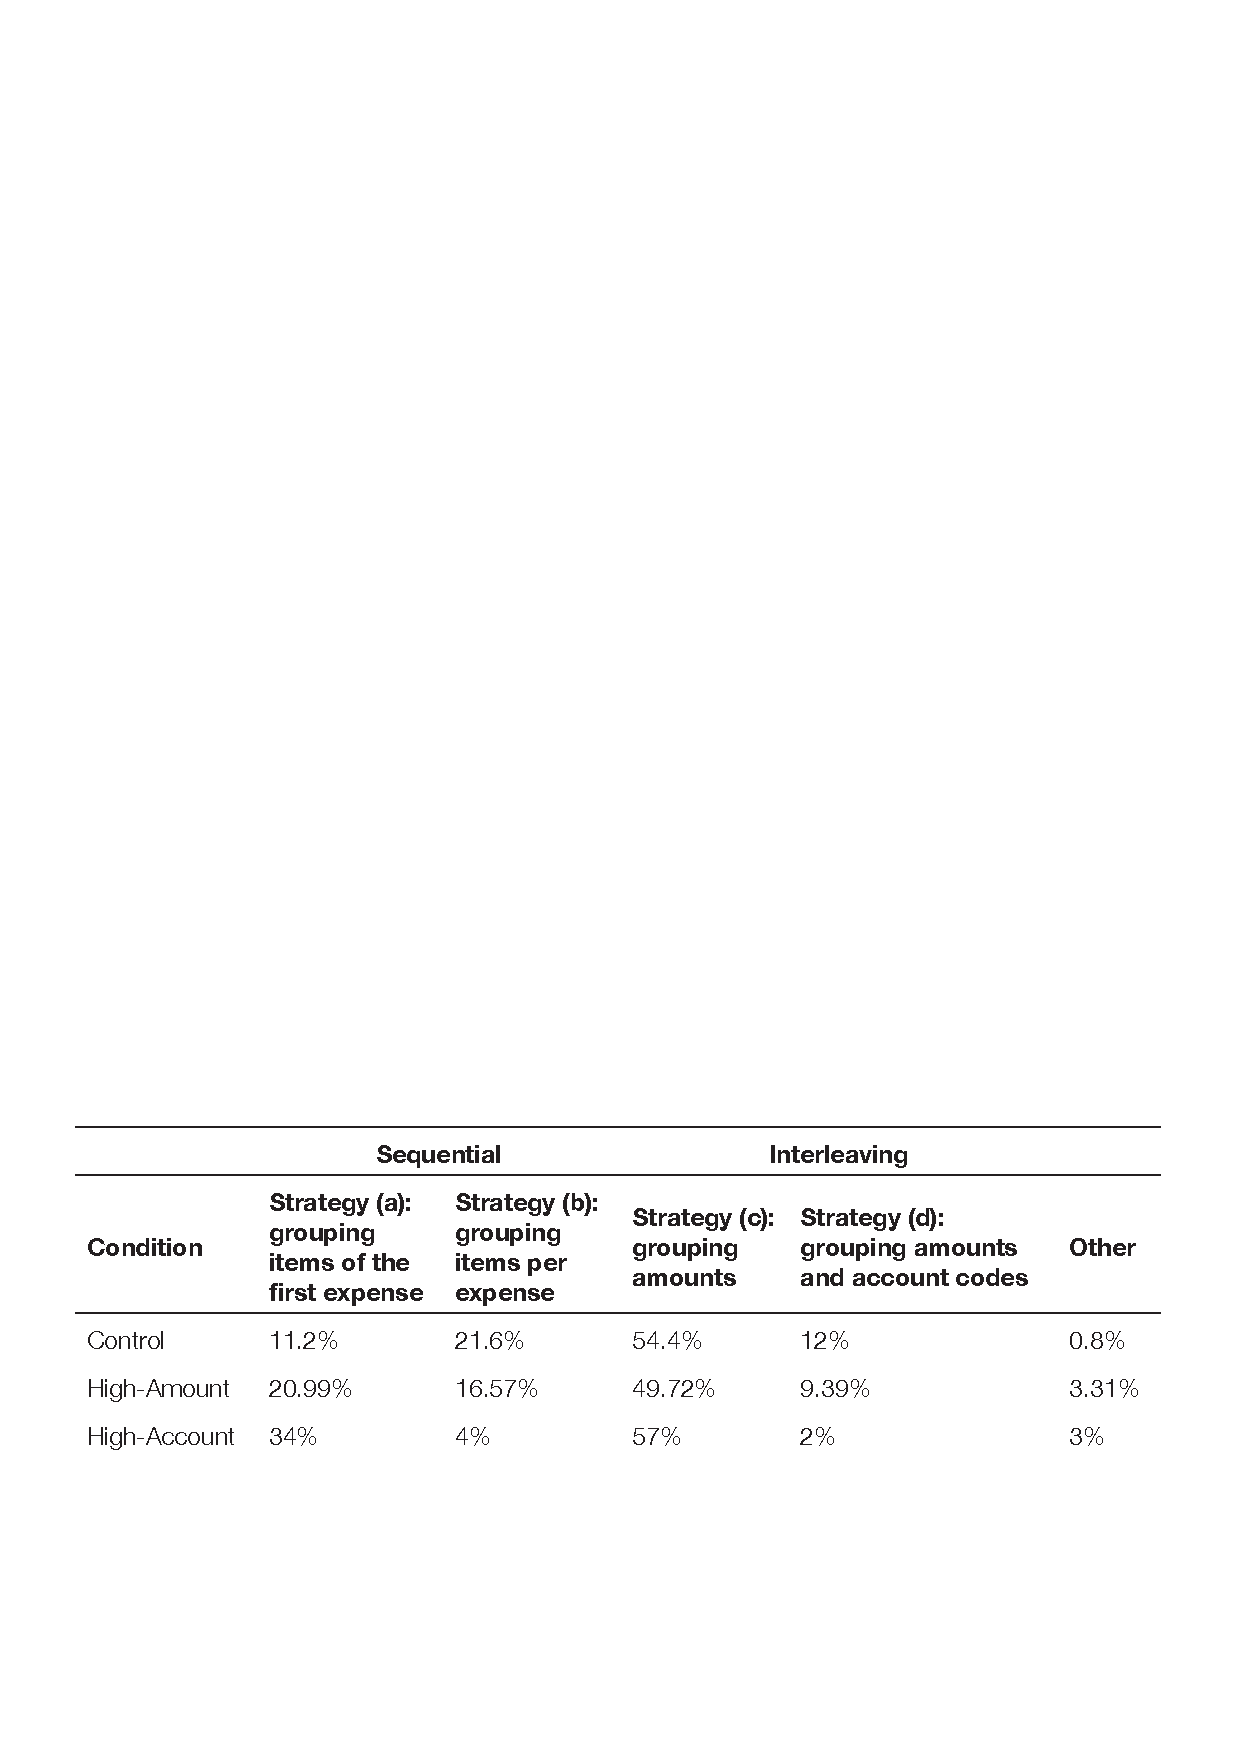
\includegraphics[width=\textwidth]{images/ch34/ch4_4-StrategyFreq.pdf}
\caption[Study 4 occurrence of most common strategies]{The occurrence of the most common strategies per condition; the most common strategy per condition is highlighted in bold. The rates are calculated by dividing the number of occurrences to the number of opportunities, e.g. a  rate of 50 percent means participants used this strategy on 50 percent of the trials. The strategies are shown graphically in Figure \ref{fig:ch34_4-groupstr}.}
          \label{tbl:ch34_4-groupstr}
\end{table}

\subsubsection{Task performance}
The High-Cost conditions had an extra time cost to overall completion time, due to the delay when switching one of the windows. Therefore, two completion times were calculated: one measure considered the actual completion time with the delay times included, and another measure considered the completion time with the delay times removed. Considering these two times, there was no difference in the time it took to complete a trial using the actual completion time,  \textit{F}(2, 30) = 0.16, \textit{p} = .90, or with the delay times removed, \textit{F}(2,30) = 1.63, \textit{p} = .20.

There were 200 data entries, so in total there were 200 opportunities for a participant to make a data entry error. The error rates were calculated as the number of errors divided by the number of entries. Though the mean error rate was higher in the Low condition (M=8.68\%, SD=10.90\%) compared to the High-AM (\textit{M}=3.77\%, \textit{SD}=2.79\%) and High-AC (\textit{M}=5.18\%, \textit{SD}=4.13\%) conditions, this difference was not statistically significant, $\chi^2$(2) = 0.41, \textit{p} = .80. 

%Considering these two times, there was no difference in the time it took to complete a trial using the actual completion time,  $\chi^2$(2) = 0.15, \textit{p} = 0.9, or with the delay times removed,  $\chi^2$(2) = 2.92, \textit{p} = 0.2. On average, with the delay times included, participants took about 29 seconds per trial across conditions.

While the above analysis shows no significant difference in the number of data entry errors, it does not give any indication of the type of errors that were made. Having insight into the type of errors can inform how to design better data entry interfaces to prevent these errors \citep{Wiseman2011}. Interleaving may increase the occurrence of specific types of errors: for instance, it has been shown that interleaving between tasks increases the likelihood of omitting task steps \citep{Back2012}. %I was therefore interested to see whether interleaving between expenses increased the number of omission errors. 
The errors were therefore categorised according to type, to see what type of errors were made across conditions. To study the type of errors that were made, \citeauthor{Wiseman2011}'s \citeyearpar{Wiseman2011} taxonomy of number entry errors was used to categorise data entry errors. This taxonomy was originally created by grouping and coding 350 number entry errors gathered during a number entry experiment. As can be seen in Figure \ref{fig:ch34_4-typeoferrors}, the most prominent error types were when participants had a digit(s) wrong (60 times), when a data entry was skipped (75 times) or when they entered a 'wrong' number, which was supposed to be entered in another data entry field (57 times): these types of errors make up for 61\% of all errors. The 'digit(s) wrong' and 'skipped' errors happened more frequently in the Low condition, but there was no remarkable difference in these types of errors between conditions,  $\chi^2$(2) = 0.27, \textit{p} = .87. 

%\citeauthor{Wiseman2011}'s \citeyearpar{Wiseman2011} taxonomy of number entry errors was used to analyse the types of data entry errors that were made. 

\begin{figure}
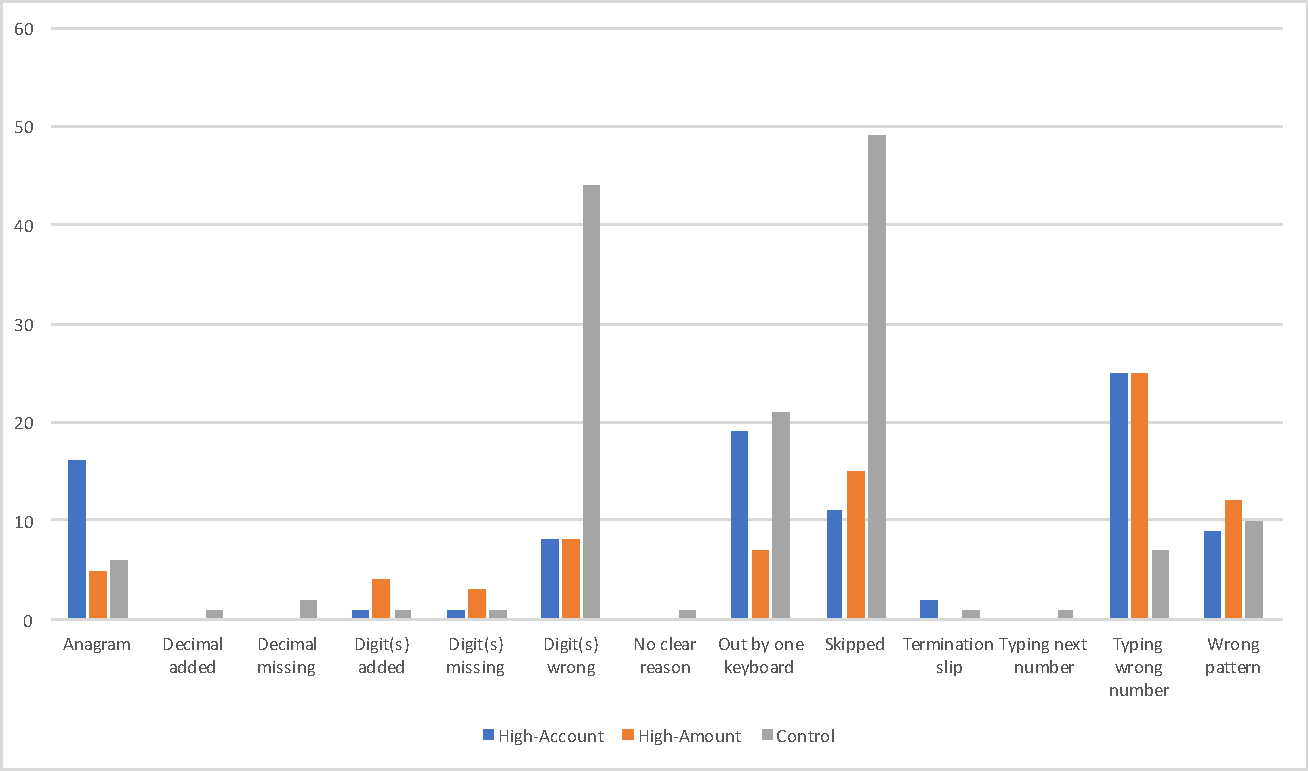
\includegraphics[width=0.85\textwidth]{images/ch34/ch34-4_TypeofErrors.pdf}
    \caption[Study 4 type of data entry errors]{The type of data entry errors made in each condition. The most common error types were when participants had a digit wrong, when a data entry was skipped, or when the wrong number was entered in an input field.}\label{fig:ch34_4-typeoferrors}
\end{figure}

\subsubsection{Qualitative findings}
After the experiment had ended, participants were debriefed and the purpose of the study was explained. Some participants reflected on their strategies and gave additional explanations behind them. While these explanations are not the main focus of analysis and only serve to complement the quantitative measures, it helps understand people's motivation behind some of the measured strategies.

Participants mentioned they adapted their strategy several times throughout the experiment, in order to find the quickest way to complete the task. Because amounts were shorter and easier to remember, five participants mentioned they tried to first view all amounts before entering them. They tried this strategy with account codes as well, but these were longer and therefore it was more difficult to memorise two items at a time. As a result, most participants ended up viewing and entering each account code one by one. This kind of behaviour is illustrated as Strategy (d) in Figure \ref{fig:ch34_4-groupstr}.

Four participants noticed that numbers re-occurred throughout the experiment. They felt it was easier to memorise a number that had already occurred earlier in the experiment, so when a trial contained a number they recognised, they would memorise this item as well as another item, before returning to the entry form. If they did not recognise the number, they would memorise one item. Furthermore, as data items had a fixed length, some participants started a trial by entering placeholders: in the amount data entry field, they placed a number consisting of four digits and a decimal point, and in the account code data entry field a number of six digits was entered. They would then visit the information windows to check which of the digits of the items they needed to change. 

\subsection{Discussion}
%Summary
The aim of this study was to understand the effect of time costs on the timing of inquiries during a data entry task. To address this aim, I created a new experimental task that involved switching between three different windows to look up and enter data. The main findings of Study \hyperref[st:Study4]{4} are:

\begin{itemize}
\item
if there were no differences in time costs, participants completed a data entry sheet in sequential order, and completed one expense before moving to the next one. 
\item
in the High-Cost conditions, people interleaved significantly more between expenses in the High-AC but not High-AM condition. 
\item
participants grouped items in all conditions, and there was no difference in number of visits between conditions.
\end{itemize}

\subsubsection{Timing of inquiries}
The findings partly support hypothesis H1: people postponed some inquiries with a high time cost, but it does not explain why participants entered the data entry sheet in sequential order in the High-AM condition. 
%The findings partly support the hypothesis that people postpone inquiries with a high time cost, but it does not explain why participants entered the data entry sheet in sequential order in the High-AM condition. 
These results can be explained when considering the order in which the data was presented, and the order in which items were entered. Across conditions, participants predominantly started each trial by entering the first cell of the data entry sheet, the amount of the first expense, regardless of whether the Amounts window had a 2-s time cost or not. However, the second item they entered was dependent upon which window had a time cost: if the Amounts window had a time cost, participants would enter an account code next. If there was a time cost when switching to the Account codes window, they would enter the second amount next.
This behaviour suggests that time costs do not influence the first visit, but do affect subsequent visits. Even though the time cost was consistent throughout the experiment, potentially the experiment was too short for participants to learn which of the windows had a delay and only adapted their strategy after they had already entered the first item. Furthermore, participants tended to stick to the same strategy they had started with throughout the experiment.

The finding that participants postpone inquiries with a high time cost is consistent with findings from Study 2 and suggests people schedule their inquiries more efficiently and effectively. Though there was no measured difference in task performance in the study, long interruptions have been shown to be more disruptive than short ones \citep{Altmann2017, Monk2008}, and leaving these until a natural breakpoint can reduce errors, as it is easier to resume a task \citep{Gould2013a, Iqbal2005}.

\subsubsection{Chunking of data items}
The findings do not support hypothesis H2: participants predominantly looked up each item one by one across conditions, and there was no difference in the number of inquiries. This finding is in contrast with Study \hyperref[st:Study3]{3} and prior work \citep{Gray2006}, where an increase in time costs reduced the number of inquiries. One item was probably the maximum amount people could reliably memorise. Some participants explained that they did try to batch and enter more items in one visit, but that they often had to go back to check if they had memorised it correctly. Furthermore, in prior studies there was no interaction involved to view information in the Low-Cost condition: information was permanently visible in the task interface. In the current study, participants always had to move their mouse and click in order to view the information pages, which may have encouraged them to try and reduce visits and chunk items even in the Low condition. The time cost affected which items participants chunked together, but not whether they chunked items or not.

\subsubsection{Transfer of strategies}
People adapted their strategies even if only some, but not all, of the information was hard to access. Exposure to time costs may have made people adapt their strategies for all inquiries. This transfer of strategies is consistent with previous research, that has shown a more memory-based strategy can be trained and transferred to other situations where the cost to access information is no longer high \citep{Patrick2014}. This study extends these findings by showing that inquiry strategies can also transfer within a task, when the user has to access multiple information sources with both a low and high time cost.

\subsubsection{Limitations}
%The study has two limitations regarding the type of data items used, and the order of data.

%Order
%All conditions had the same order in which data was presented on the data entry sheet, as well as the same order in which the windows were shown in the top menu. 
The results suggest that the order in which data was presented may have influenced the order in which people entered data: across all conditions, participants mostly started a task by entering the first data item. An increased time cost affected subsequent items that were entered after the first item. Future studies could be done to investigate whether changing the order has an effect on people's inquiry strategies.

% As the results show, the effect of time costs was only shown in the High-Account condition, which may have partly been caused because of a difference in data item: account codes were longer and more difficult to memorise, which may have been an additional time cost, that encouraged people to first look up amounts.

\subsection{Conclusion}
Taken together, the findings from this study suggest that people avoid time costs by postponing some inquiries with an increased time cost, and addressing inquiries with a low time cost first. In contrast, if all inquiries have the same time cost, participants predominantly filled in a data entry sheet in sequential order. They completed one expense first, before moving to the next one. 

In the current study, both expenses were shown in the same window. Even though switching between expenses was labelled as an 'interleaving' strategy in the study, the expenses were part of one form, and could be seen as part of the same task. What we do not know from Study \hyperref[st:Study4]{4} is whether participants will also avoid time costs of inquiries by interleaving between two data entry tasks separated over two different windows. Based on the results of the current study, the hypothesis is made that a difference in time costs makes people more likely to interleave between different data entry tasks to enter items with a low time cost first. This hypothesis is tested in Study \hyperref[st:Study5]{5}.

%The aim of this study was to investigate the effect of time costs on the number, duration and timing of inquiries from multiple sources. We learn from this study that people avoid time costs by postponing some inquiries with an increased time cost. If there were no differences in time costs, people completed a data entry sheet in sequential order, and completed one expense before moving to the next one. 

%In this study, both expenses were shown on the same window, and could be seen as part of the same task. 

\section{Study 5: Inquiries for multiple tasks}\label{st:Study5}
\subsection{Introduction}
So far, Study \hyperref[st:Study3]{3} has shown that people avoid time costs by reducing the number of inquiries, and Study \hyperref[st:Study4]{4} suggested that people avoid time costs by postponing inquiries with a high time cost. In these studies, people were only presented with one task at a time. Workers in Study \hyperref[st:Study2]{2} often dealt with several data entry tasks and windows at a time, and had to be careful not to enter information in the wrong windows. How would people deal with time costs when they have to coordinate multiple tasks? Participants in Study \hyperref[st:Study1]{1} and \hyperref[st:Study2]{2} avoided switches to tasks that were completely unrelated to their data entry work, but people may switch between similar data entry tasks if it makes them faster. For instance, upon opening a spreadsheet that takes time to retrieve, it may be more efficient to enter the account codes from that spreadsheet for multiple tasks. However, multitasking can also be prone to errors \citep{Carrier2015}.

Prior research, studying the effect of time costs on multitasking in a hospital setting, found that increased time costs reduces multitasking. \citet{Back2012} conducted a lab experiment where participants had to enter information from a prescription form into two simulated infusion pumps. For each pump, they had to enter two types of information: the medication dose and the time duration. If the form was physically further away from the pumps, participants more often completed one pump before starting another and as a result made fewer errors in omitting a task step. The higher access cost had the effect that participants memorised and chunked information on the form according to the pump rather than type of information, which reduced multitasking.

However, in Back et al.'s study, all information was located on one information source, and participants incurred a single cost to access it. People therefore chunked information to memorise as much information per visit as possible, so that they did not have to revisit the source too often. It is unclear what the effect of time costs is in scenarios where people do not have to get multiple information items from one source, but rather information from multiple sources. How do people prioritise which information to look up first? Do they still complete looking up information for one task first, before starting another task?

The aim of Study \hyperref[st:Study5]{5} is to test whether the effect of time costs, as found in Study \hyperref[st:Study4]{4}, extend to a multi-task setup. Participants were asked to complete an experiment similar to the task in Study \hyperref[st:Study4]{4}, but had to complete two (of the same) data entry tasks per trial. The following hypothesis is made:

\begin{itemize}
\item [H1.]
Participants in the Low condition will enter items from one data entry task first, before entering the second task. Participants in the High-Cost conditions will interleave between expenses and enter the Low-Cost items first, and postpone entering the High-Cost items.
\end{itemize}

\subsection{Method}
\subsubsection{Participants}
Thirty-nine participants (32 female, seven male), ranging from 18-46 years (M = 25, SD= 8) took part in the experiment. They were recruited from a university subject pool and received $\pounds$4 for their participation.

\subsubsection{Materials}
The experimental task was similar to the one used in Study \hyperref[st:Study4]{4} but differed in one aspect. Instead of filling in one data entry form per trial, participants had to complete two sheets per trial, which were shown on two different windows (see Figure \ref{fig:ch34_5-tasklayout}). Each data entry sheet contained one expense, and participants completed the trial by entering the amount and account code for each sheet. The aim of this follow-up study was to investigate if differences in time costs of the two information windows makes people more likely to interleave between two separate data entry tasks.

\begin{figure}
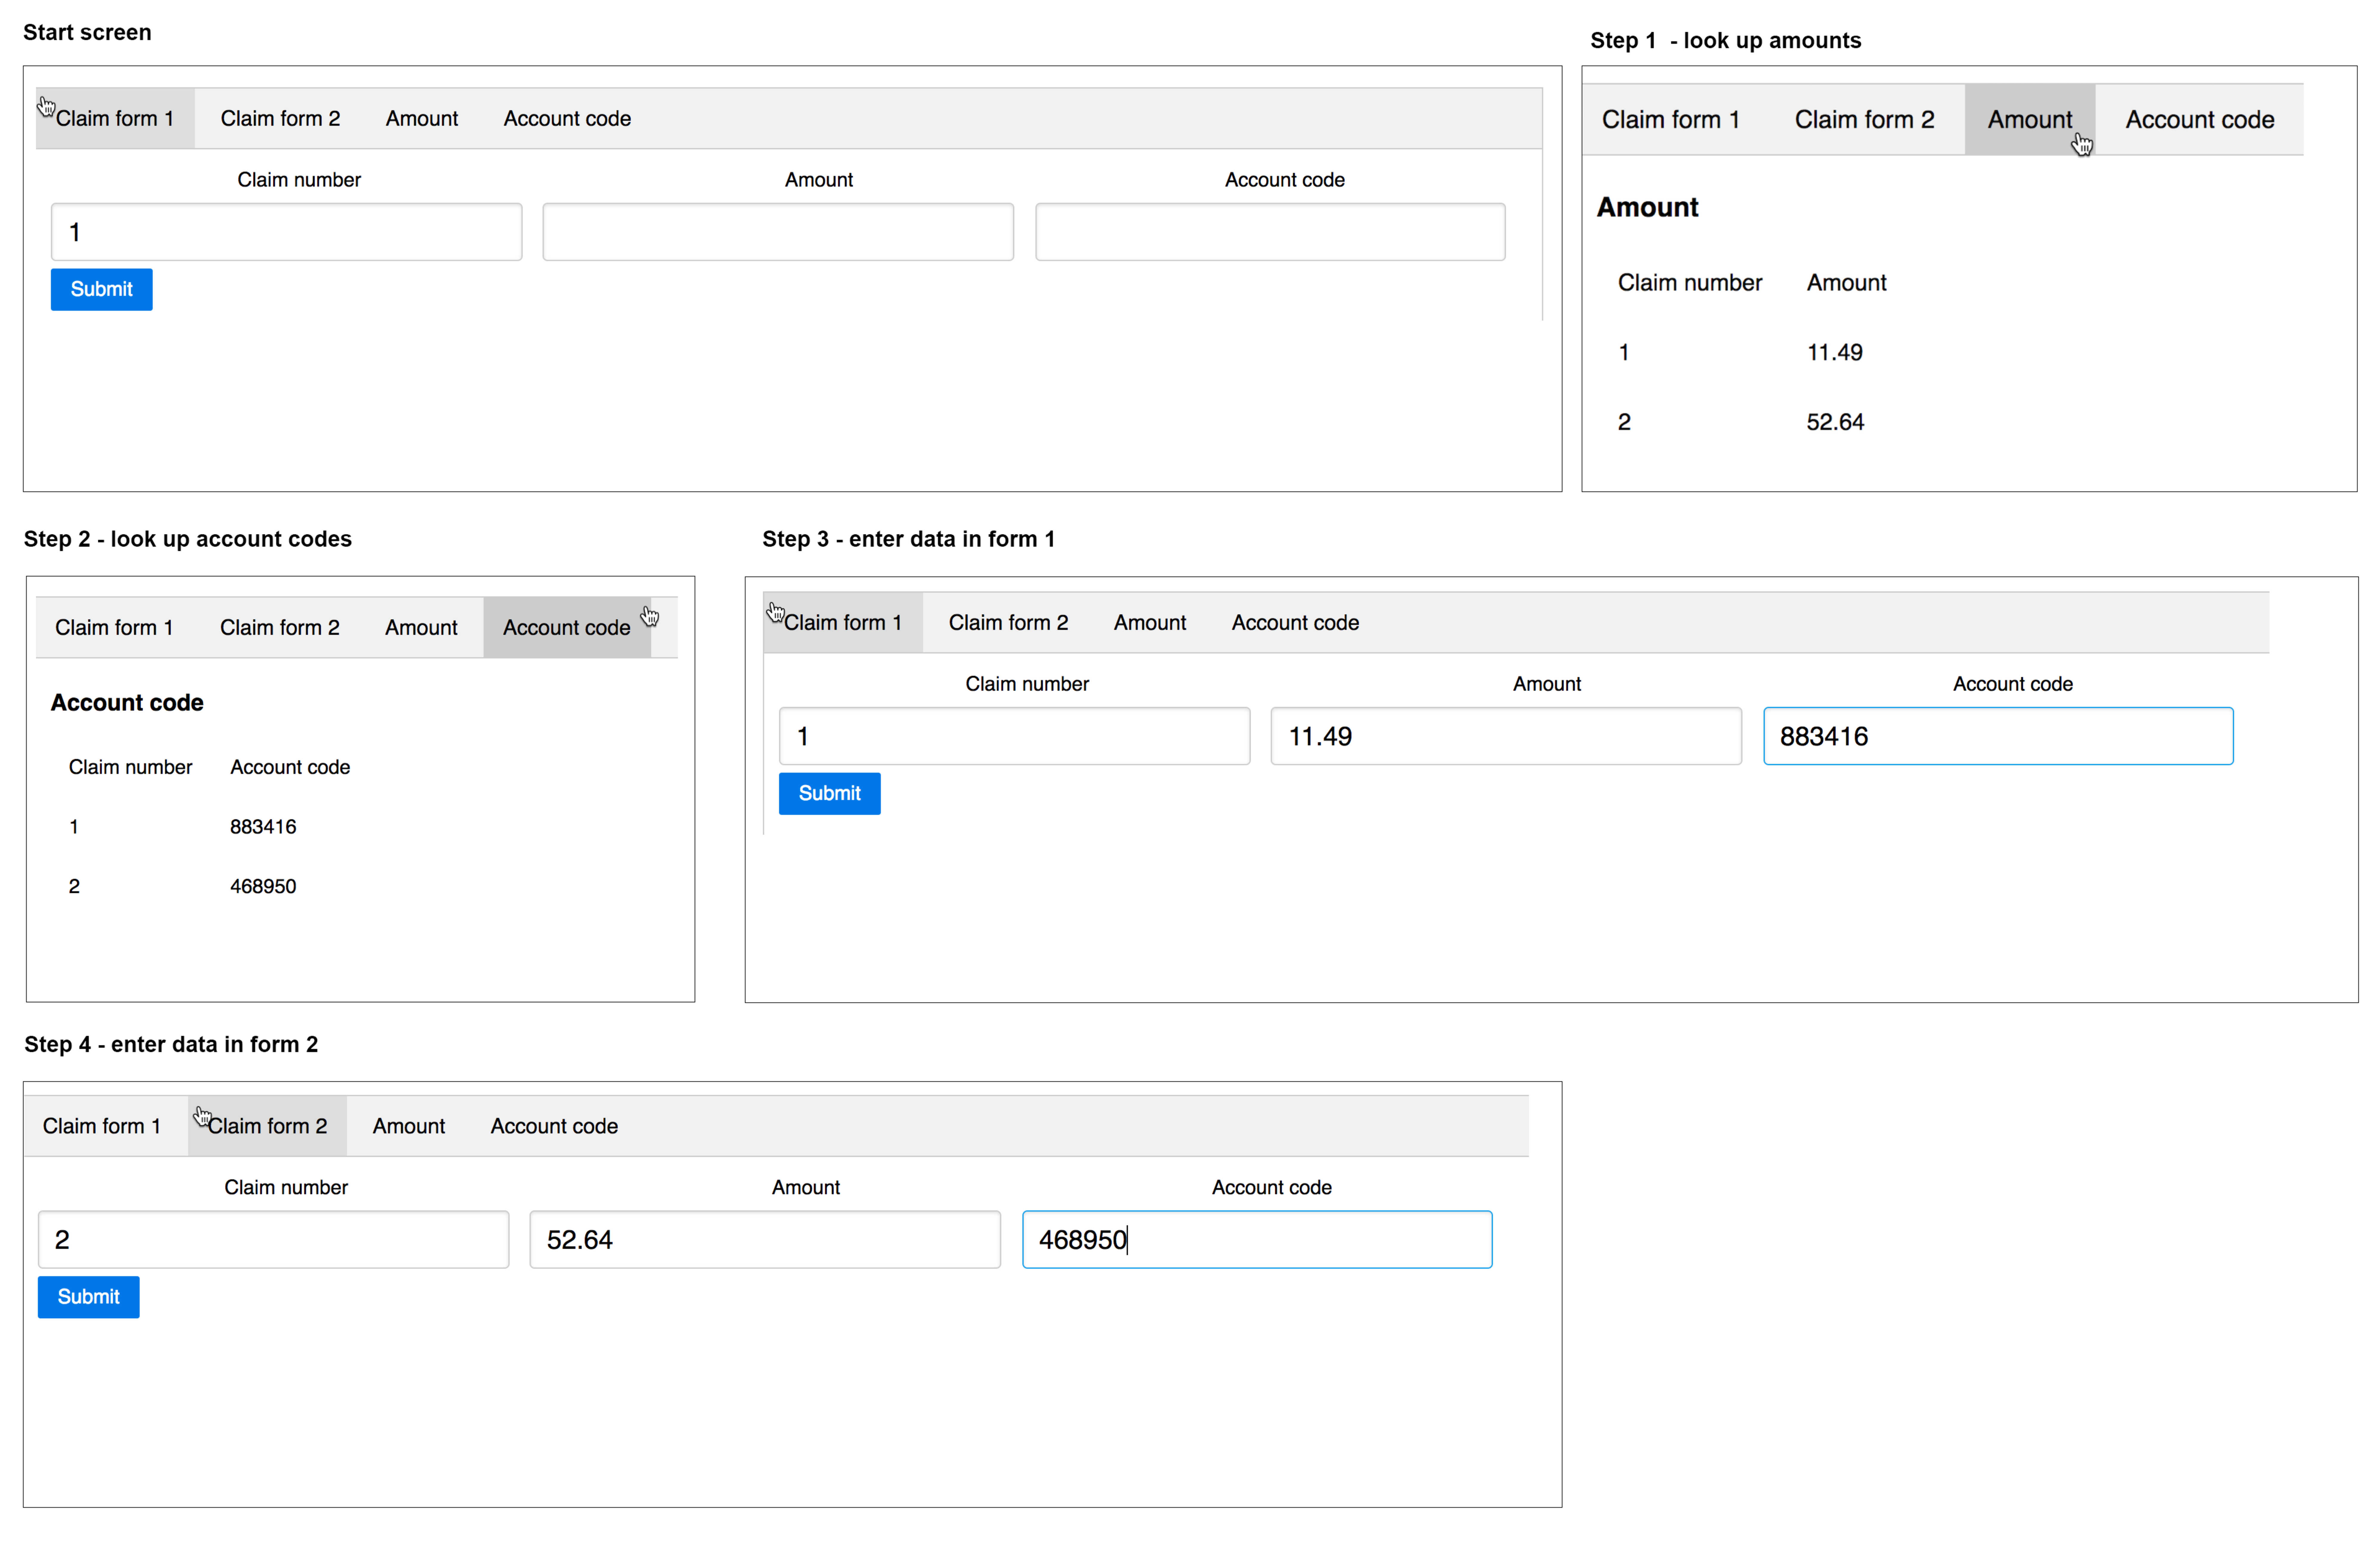
\includegraphics[width=\textwidth]{images/ch34/ch34-5_Tasksequence.pdf}
    \caption[Study 5 data entry task layout]{Participants had to enter two data entry tasks per trial, each containing two items. Each trial started by showing the first data entry form. As in Study 4, the data items for both tasks were retrieved from a separate Amounts window (Step 1) and entering the items for the first expense (Step 2), and the second expense (Step 3). Participants had to repeat Steps 2 and 3 for the account codes, before submitting the data entries and moving on to the next trial. The participant could switch back and forth between windows as often as is needed}\label{fig:ch34_5-tasklayout}
\end{figure}

\subsubsection{Design}
The experiment was a between-participants design with the presence of a delay as the independent variable. 
As in Study \hyperref[st:Study4]{4}, in the \textit{Low-Amount, Low-Account} (Low) condition, there were no delays in opening any of the windows. In the \textit{High-Amount, Low-Account} (High-AM) condition, there was a 2-s delay when opening the Amount window, and no delay when opening the Account window. In the \textit{Low-Amount, High-Account} (High-AC) condition, there was no delay when opening the Amount window, and a 2-s delay when opening the Account window. There were no delays in opening the data entry form in any of the conditions 
The main dependent variable was whether participants interleaved between sheets or not: did participants enter the data items in sequential order, or did they interleave between the two sheets? If participants entered the amount and account code of one sheet before entering the other sheet, this was considered a sequential order. If participants entered amounts of each sheet first, followed by entering the account codes or vice versa, this was considered interleaving. All window switches and key presses were recorded to determine in which order data was entered. Window switches were recorded to capture when and how often a participant looked up the data items. Other dependent variables were trial completion time, data entry error rate, and type of errors.

%As in Study 4, in the Control condition there were no delays in opening the windows. In the High-Amount condition, there was a delay in opening the window with amounts. In the High-Account condition, there was a delay in opening the window with account codes. 

\subsubsection{Procedure}
The experimental setup was similar to Study \hyperref[st:Study4]{4}. For each experimental trial, participants had to enter four data items: they had to complete two forms with two entries each, an account code and an amount. For each experimental trial, participants had to enter four data items, two for each sheet. It was explained that they could use any strategy they wanted, but that it was important to complete both sheets before continuing to the next trial. Participants first completed two practice trials to familiarise themselves with the task, and data from the practice trials were excluded from the analysis. The experiment took approximately 30 minutes.

\subsubsection{Data analysis}
%Participants again predominantly started a trial by viewing and entering the amount of the first expense. If the participant then proceeded to view and enter the account code, this strategy was labelled as a sequential strategy. If the participant proceeded to enter, or view and enter, the amount of the second expense, the trial was labelled as an interleaving strategy. 
The main interest of Study \hyperref[st:Study5]{5} was to see whether people interleaved between tasks or not, and not the specific order of individual actions (e.g. did participants enter multiple items after a single visit to a data window). Strategies are therefore not presented here in the same detail as in Study \hyperref[st:Study4]{4} (see section \ref{sec:ch34-StrategyFreq}). Trials were categorised into an interleaving or sequential category. On a trial-by-trial basis, it was also considered whether people started the trial by visiting and entering a High-Cost or Low-Cost data item.

\subsection{Results}
Table \ref{tbl:ch34_5-means} shows a summary of the results of all three conditions for the dependent variables. Kruskal-Wallis tests were carried out to test if there were significant differences in interleaving rate, number and duration of visits, and error rate between the conditions, as these measures did not follow a normal distribution. 
A Shapiro-Wilk test suggested that the trial completion times did follow a normal distribution, \textit{W} = 0.94, \textit{p} = .05, so a one-way ANOVA was used to test any differences in trial completion time. A p-value of 0.05 was used for assessing the significance of all statistical tests. 

\subsubsection{Cleaning up the data}
Three participants were removed from the data due to extreme values on performance measures.
P28 and P23 made at least one error on every trial. They made 118 and 153 errors out of 200 error opportunities, respectively. P26's session was terminated before the end had been reached, as 45 minutes had passed. This participant spent on average 65 seconds per trial, which is twice as long as the mean trial time of other participants. These three participants were considered outliers and did not seem to engage with the study, and their data was removed from the dataset. Data of the remaining 39 participants was taken into the data analysis.

\begin{table}
 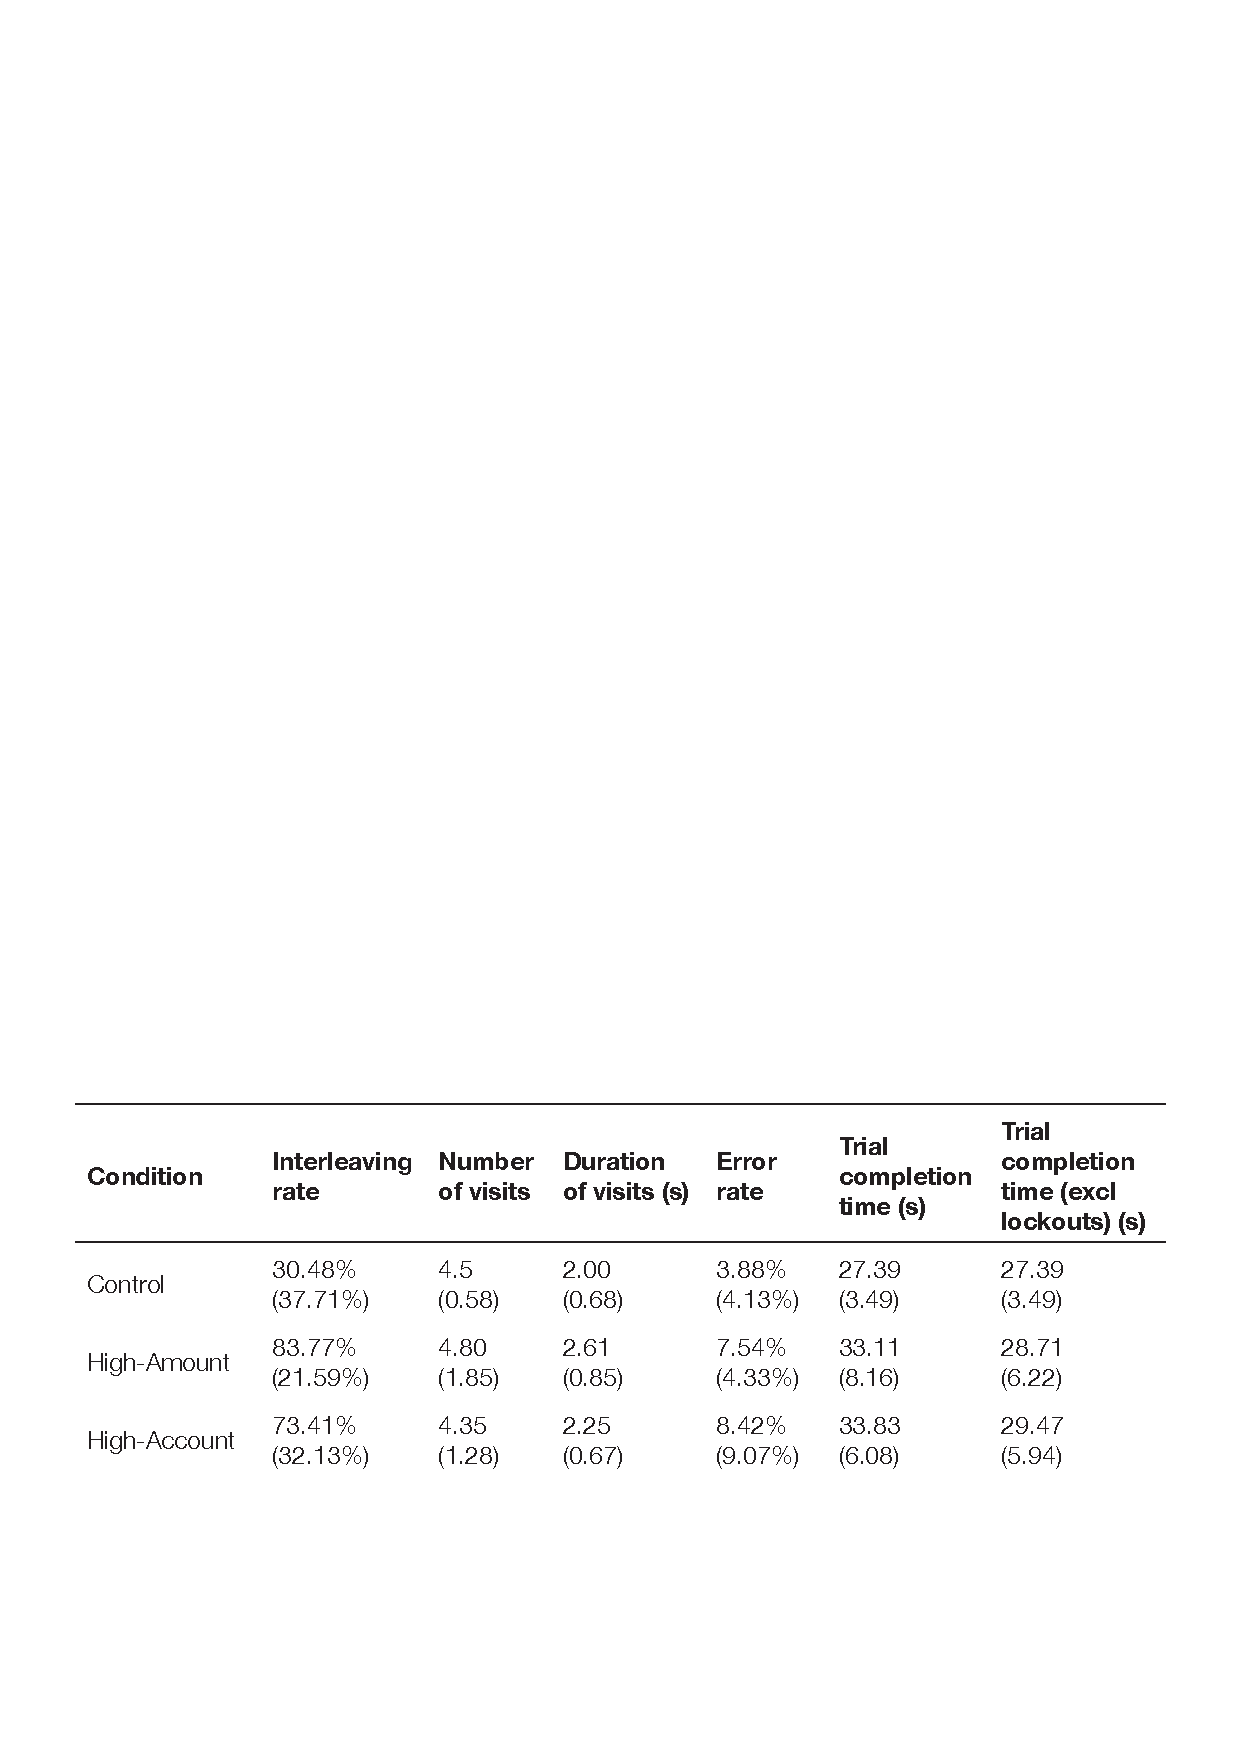
\includegraphics[width=\textwidth]{images/ch34/ch34_5-means.pdf}
\caption[Study 5 means and SDs of dependent measures]{The means (and standard deviations) of all dependent measures for each condition. The rates are calculated by dividing the number of occurrences to the number of opportunities, e.g. an interleaving rate of 50 percent means participants interleaved on 50 percent of trials.}
\label{tbl:ch34_5-means}
\end{table}

\subsubsection{Interleaving strategies}
A trial was labelled as 'interleaving' if the participant started entering one data entry sheet, but interleaved to entering items on the other sheet before completing the first one. The interleaving rate for each condition was calculated by dividing the number of trials where people interleaved by the number of total trials. 

Participants interleaved most often between data entry sheets in the High-AC (\textit{M} = 73.41\%, \textit{SD} = 32.13\%) and High-AM (\textit{M} = 83.77\%, \textit{SD} = 21.59\% ) conditions compared to the Low (\textit{M} = 30.48\%, \textit{SD} = 37.71\%) condition, $\chi^2$(2) = 11.13, \textit{p} < .01. A post-hoc comparison showed there was a difference between the Low and the High-AM (\textit{p} < .01) and High-AC (\textit{p} = .01) conditions, and no difference between the High-AC condition and the High-AM (\textit{p} = .40) conditions. The median interleaving rate was 14.58\% for the Low condition, 94.00\% for the High-AM condition, and 89.58\% for the High-AC condition. The boxplots in Figure \ref{fig:ch34_5-boxplots} show the variability of interleaving rates across conditions. 

As can be seen in Figure \ref{fig:ch34_5-linechart}, which shows the distribution of interleaving rates, all participants in the High-Cost conditions interleaved on at least a part of the trials: the lines of the High-Cost conditions have a frequency of 0 (participants) at an interleaving rate of 0\%. The Low condition has a flat line with no peaks, indicating that interleaving rates in this condition were evenly distributed: participants interleaved on zero, a portion, as well as all of the trials.

\begin{figure}
 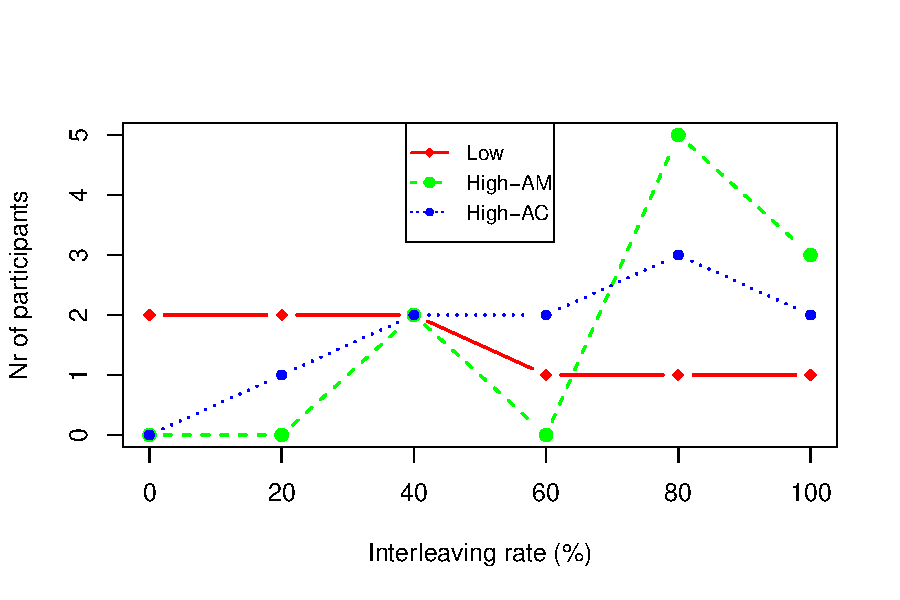
\includegraphics[width=\textwidth]{images/ch34/ch34-5_linechart.pdf}
\caption[Study 5 frequency of interleaving rates]{Line graph showing the frequency of interleaving rates for each condition. It can be seen that in the Low condition, the line is even, which means that an even distribution of participants interleaved on all, a portion, or all trials. The lines of the High-Cost conditions peak at the right end, which means most participants in these conditions interleaved on at least a portion if not 100\% of all trials.}
\label{fig:ch34_5-linechart}
\end{figure}

On the majority of trials where participants interleaved (81.95\%), they visited and entered Low-Cost items first. On a small subset of trials, participants interleaved by entering High-Cost items first: on 2.77\% of the interleaving trials participants entered High-Cost account codes first, and on 15.28\% of these trials participants entered High-Cost amounts first. 

\begin{figure}
 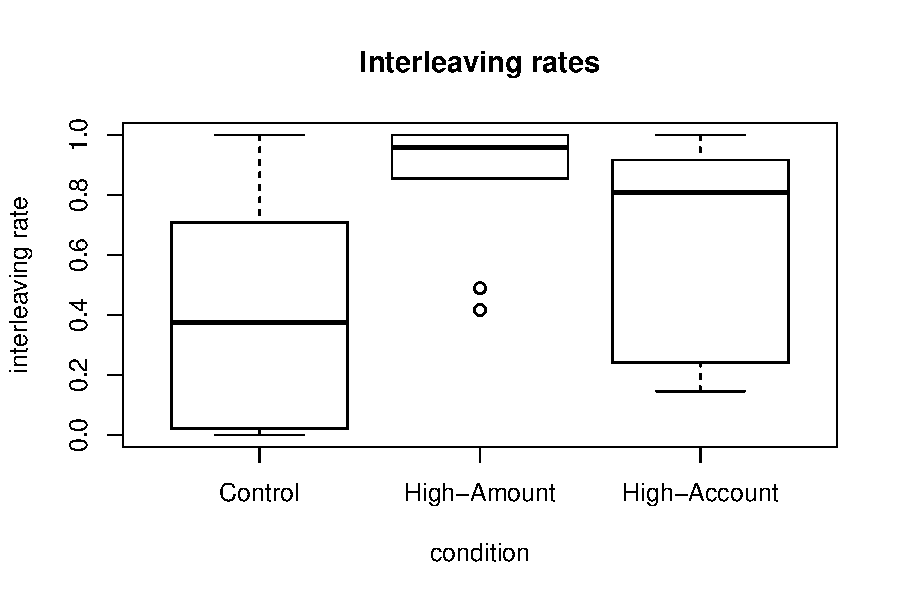
\includegraphics[width=0.6\textwidth]{images/ch34/ch4_5-boxplot.pdf}
\caption[Study 5 boxplot of interleaving rates]{Boxplot of interleaving rates in each condition.}
\label{fig:ch34_5-boxplots}
\end{figure}

\subsubsection{Number and duration of visits}
As in Study \hyperref[st:Study4]{4}, participants made on average four visits per trial, i.e. one visit per data entry. There was no difference in the number of visits, $\chi^2$(2) = 1.59, \textit{p} = .50. Participants made significantly shorter visits in the Low (\textit{M} = 2.00s, \textit{SD} = 0.68s) condition compared to the High-AC condition (\textit{M} = 2.25s, \textit{SD} = 0.67s) compared to the High-AM (\textit{M} = 2.61s, \textit{SD} = 0.85s) and  $\chi^2$(2) = 6.14, \textit{p} = .04. Post-hoc comparisons found a significant difference between  the High-AM and the Low (\textit{p} = .02) conditions, but not between High-AC and Low conditions (\textit{p} = .20) or the High-AC and the High-AM (\textit{p} = .20).

\subsubsection{Task performance}
Two completion times were calculated: one measure considered the actual completion time with the delay times included, and another measure considered the completion time with the delay times removed. When comparing the actual completion time including lockouts, participants were significantly faster in the Low condition (\textit{M} = 27.39, \textit{SD} = 3.49s) than the High-AC (\textit{M} = 33.83s, \textit{SD} = 6.08s) or High-AM (\textit{M} = 33.11s, \textit{SD} = 8.16s) conditions, \textit{F}(2, 36) = 6.73, \textit{p} < .01. With the lockout times removed, the difference is no longer significant, \textit{F}(2, 36) = 0.66, \textit{p} = .50.

There were 200 data entries, so in total there were 200 opportunities for a participant to make a data entry error. The error rates were calculated as the number of errors divided by the number of entries. There was a marginal though not significant effect of time cost on error rate, $\chi^2$(2) = 5.37, \textit{p} = .06. The mean error rate was marginally higher in the High-AC condition (\textit{M}= 8.42\%, \textit{SD} = 9.08\%) compared with the High-AM (\textit{M}=7.54\%, \textit{SD}=4.33\%) and Low (\textit{M} = 3.88\%, \textit{SD} = 4.13\%) conditions. 

%When comparing the actual completion time including lockouts, participants were significantly faster in the Low condition (\textit{M} = 27.39, \textit{SD} = 3.49s) than the High-AC (\textit{M} = 33.83s, \textit{SD} = 6.08s) or High-AM (\textit{M} = 33.11s, \textit{SD} = 8.16s) conditions,  $\chi^2$(2) = 8.52, \textit{p} = 0.01. With the lockout times removed, the difference is no longer significant, $\chi^2$(2) = 1.61, \textit{p} = 0.4.

\begin{figure}
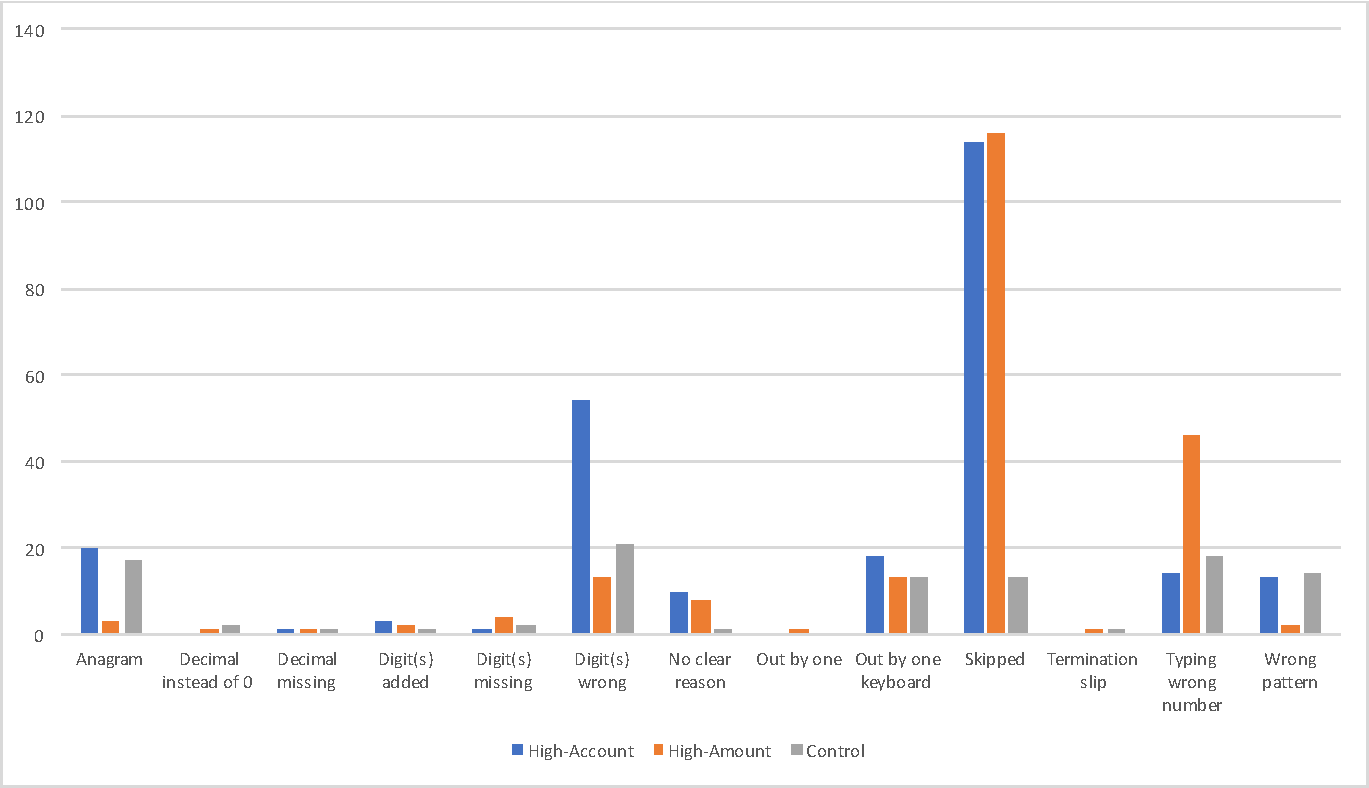
\includegraphics[width=0.85\textwidth]{images/ch34/ch34-5_TypeofErrors.pdf}
    \caption[Study 5 type of data entry errors]{The type of data entry errors made in each condition. It can be seen that skipped errors occurred more often in the High-Cost conditions, in which people interleaved more often.}\label{fig:ch34_5-typeoferrors}
\end{figure}

The type of errors can be seen in Figure \ref{fig:ch34_5-typeoferrors}. The most common error type was when a data entry was skipped: this happened 243 times. %Table 1 shows the number of skipped errors for each condition. 
In the Low condition this type of error occurred 16 times. The error happened more frequently in the High-Cost conditions: in the High-AC condition it happened 114 times, and in the High-AM condition it happened 116 times.
Typing the correct number but in the wrong field happened 78 times. This error happened 18 times in the Low condition, 14 times in the High-AC and 46 times in the High-AM condition.
When comparing across conditions, these two types of errors happened on a significantly higher proportion of data entries in the High-AC (\textit{M} = 4.58\%, \textit{SD} = 3.6\%) and High-AM (\textit{M} = 6.54\%, \textit{SD} = 5.01\%) compared with the Low condition (\textit{M} = 1.23\%, \textit{SD} = 1.82\%),  $\chi^2$(2) = 11.29, \textit{p} < .01.  A post-hoc comparison showed there was a difference between the Low and the High-AM (\textit{p} < .01) and High-AC (\textit{p} = .01) conditions, and no difference between the High-AC condition and the High-AM (\textit{p} = .40) conditions.


\subsection{Discussion}
%Effect of time costs
The results show that participants in High-Cost conditions interleaved more between expenses, and made more omission errors, which means a data entry was skipped. The study further supports the notion that people avoid time costs and try to minimise time by postponing some inquiries with an increased time cost, and it demonstrates that this effect of time costs extends beyond a single task setup.
%Though interleaving also happened in the Control condition, it happened significantly more often in the High-Cost conditions. 

The findings support hypothesis H1: participants in the High-Cost conditions entered Low-Cost items of each expense first, and postponed entering the High-Cost items. On a small subset of trials, participants interleaved but instead of entering Low-Cost items, they chose to enter High-Cost items first. One explanation for this behaviour is the order in which data was presented, which was briefly discussed earlier for Study \hyperref[st:Study4]{4}. In the High-AM condition, participants may at times have chosen to start a trial by viewing and entering the first data item, which was the amount of the first expense, even though there was a time cost of accessing this item. Another possible explanation is that participants were trying out different strategies, to learn the most efficient strategy for them. 

%avoided time costs by entering items with a low cost first, which meant they interleaved between expenses and entered items of each expense that had a low cost first. 

The finding that people increase their interleaving behaviour to avoid time costs is consistent with the soft constraints hypothesis that people adapt their strategies to millisecond changes in an interface \citep{Charman2003, Gray2004}. In previous studies, it was shown how time costs affect the number of steps taken to complete a task \citep{Gray2006}. Study 4 and 5 contribute to this line of work by showing time costs also affect the order of steps in a routine task.

%Interleaving
The finding that participants interleaved more as time costs increased, contrasts with \citet{Back2012}, who found that an increase in time costs made people less likely to interleave between two data entry tasks. This contrast may be due to the presentation of the information. In \citet{Back2012}'s study, people had to retrieve all information for both data entry tasks from one sheet. If the sheet was nearby, participants read one item at a time, and interleaved between tasks on 59\% of the trials.  As the cost to access this source increased, they chunked the data items associated with one task, and then after completing this task, returned to the source to chunk data items for the second task. 

%Contrary to prior research, there was no difference in number or duration of visits. Across conditions, participants made one switch per data entry which is probably the maximum amount people can reliably hold in short-term memory. 

%Contribution and implication
This study contributes to our understanding of how time costs affect task switching behaviour, and can have implications for tools aimed to minimise task switches. In the current study, there was only a time cost when switching to one of the information sources, but not when switching between tasks. The results showed that people try to avoid switching to something with a high cost. Therefore, adding a cost when switching between tasks may encourage people to complete one task, before switching to another task.

\subsubsection{Limitations}
Even though the two data entry tasks were separated on different windows, participants may still have felt it was part of the same activity, as the two data entry tasks were shown in the same interface and browser window. Study \hyperref[st:Study2]{2} suggests that even though people tried to avoid task switches, they  made frequent switches that were seen as part of the activity. For Study \hyperref[st:Study6]{6}, participants will have to switch between different browser windows, to investigate window switching behaviour. 

%Using different items
The experimental task in Studies \hyperref[st:Study4]{4} and \hyperref[st:Study5]{5} was modelled on an expenses task, and the numbers to be entered were similar to data items used for that type of task: financial amounts and account codes. To ensure that any measured differences in inquiry strategies were due to time costs associated with an inquiry, rather than the type of data item that was being accessed, there were two conditions with an increased time cost: in the High-AM condition, there was a time cost to access the Amounts window, and in the High-AC condition, there was a time cost to access the Account window. To simplify the task, the experimental design in Study \hyperref[st:Study6]{6} in the next chapter was adapted so participants only had to enter one type of data item. 

\section{Summary of Chapter 4}
The aim of this chapter was to investigate the effect of time costs on the number, duration and timing of inquiries for a data entry task. Study \hyperref[st:Study3]{3} showed that if people retrieve all data from the same source, they will reduce switches between entering and looking up data if the access costs to this source increases. As it took more time to access, offloading behaviour was observed as well, and several participants prepared items they were going to need nearby, but did not use them yet. Study \hyperref[st:Study4]{4} further demonstrates that when people have to retrieve data from multiple sources, they collect and group items that are quick to access first, and leave items that take longer to access until the end. Study \hyperref[st:Study5]{5} demonstrated the robustness of the effect of time costs in a multi-task setup: when dealing with two data entry tasks, people still predominantly entered items with a low time cost first, which meant they interleaved between tasks to enter items with low costs first. As a result, participants made more skipping errors and submitted tasks before they had completed entering all the items. 

These studies contribute to our understanding of the effect of time costs on self-interruption behaviour to collect information: if people know the expected time duration of an interruption, they make fewer interruptions that are long and postpone these switches. Comparing the results reported in this chapter with the results from Chapter \ref{ch:12}, office workers in Study \hyperref[st:Study2]{2} took time costs into account in a similar manner when managing physical interruptions, but not when managing digital interruptions: these were addressed immediately as participants presumed these to be quick. This behaviour suggests that people may not be aware of time costs of digital interruptions in a naturalistic setting. In the experiments in this chapter, time costs were manipulated in a specific way: a time delay was added to the interface to reveal information. In practice, the time spent on an inquiry may be because of the time to access it, but also because of time spent searching for information, or people get distracted, and further self-interrupt to other activities. These factors may further make it difficult for participants to learn the time costs associated with interruptions and adapt their self-interruption behaviour. 

%Mixed media
%The studies presented in this chapter only looked at digital inquiries. Future work could be done to compare the use of physical and digital sources in a controlled setting. For example, a future study could investigate how people prioritise digital and physical inquiries with different time costs, and whether people address physical or digital inquiries first.  
%Findings from Study 2 suggested that people are less aware of time spent on digital interruptions compared to physical interruptions. The studies aimed to investigate, if people are able to learn the time costs of digital interruptions in a controlled setting, they do take this into account. 

The studies so far have shown that people try to minimise time to complete their data entry work in an efficient way, but are not aware of the time they spend away from their task looking up information required for the task. The next chapter explores whether a design intervention showing people how long they go away for can make people more aware of these digital interruptions, and whether this has an effect on interruption strategies and task performance.